\documentclass{article}

% if you need to pass options to natbib, use, e.g.:
%     \PassOptionsToPackage{numbers, compress}{natbib}
% before loading neurips_2020

% ready for submission

% to compile a preprint version, e.g., for submission to arXiv, add add the
% [preprint] option:
%     \usepackage[preprint]{neurips_2020}

% to compile a camera-ready version, add the [final] option, e.g.:
%     \usepackage[final]{neurips_2020}

% to avoid loading the natbib package, add option nonatbib:
    %  \usepackage[nonatbib]{neurips_2020}

\usepackage[utf8]{inputenc} % allow utf-8 input
\usepackage[T1]{fontenc}    % use 8-bit T1 fonts
% \usepackage{hyperref}       % hyperlinks
\usepackage{url}            % simple URL typesetting
\usepackage{booktabs}       % professional-quality tables
\usepackage{amsfonts}       % blackboard math symbols
\usepackage{nicefrac}       % compact symbols for 1/2, etc.
\usepackage{microtype}      % microtypography

\usepackage{graphicx}
\usepackage{subcaption}
\usepackage{makecell,multirow} %

\usepackage{xcolor}
\definecolor{niceblue}{rgb}{0.0,0.19,0.56}
\usepackage[breaklinks]{hyperref}
\def\UrlBreaks{\do\/\do-}
\usepackage{breakurl}
\hypersetup{colorlinks,linkcolor={blue},citecolor={niceblue},urlcolor={blue}}
\usepackage{amsmath}
\newcommand{\theHalgorithm}{\arabic{algorithm}}
\usepackage{caption}
\usepackage{mwe}

\usepackage{algorithm}
\usepackage{algorithmic}
\usepackage[final,nonatbib]{neurips_2021}
\usepackage{xcolor}
\usepackage{enumitem}
% \usepackage{emoji}
\usepackage{optidef}
\usepackage{soul}
\usepackage{textcomp}  % Required for encoding \textbigcircle
\usepackage{scalerel}  % Required for emoji \scalerel
\sethlcolor{lightgray}
\def\hourglass{\scalerel*{
\includegraphics{resources/emoji/23f3.pdf}}{\textrm{\textbigcircle}}}
\def\checkbox{\scalerel*{
\includegraphics{resources/emoji/2705.pdf}}{\textrm{\textbigcircle}}}
\DeclareSymbolFont{matha}{OML}{txmi}{m}{it}% txfonts
\DeclareMathSymbol{\varv}{\mathord}{matha}{118}

\newcommand{\block}[1]{%
  \raisebox{\dimexpr(\fontcharht\font`X-1em)/2}{\rule{1em}{#1\dimexpr1em/8}}%
}
\DeclareUnicodeCharacter{2581}{\block{1}}


\title{Distributed Deep Learning In Open Collaborations}

\author{%
  Michael Diskin\thanks{Equal contribution. Correspondence to \texttt{mryabinin0@gmail.com}\newline Detailed author contributions are listed \hyperref[sec:contributions]{at the end} of the work.}\textsuperscript{\hspace{0.6em}$\dag\heartsuit$}
   \And
   Alexey Bukhtiyarov\footnotemark[1]\textsuperscript{\hspace{0.6em}$\dag\clubsuit$}
   \And
   Max Ryabinin\footnotemark[1]\textsuperscript{\hspace{0.6em}$\dag\heartsuit$}
   \AND
   Lucile Saulnier\textsuperscript{$\ddag$}
   \And
   Quentin Lhoest\textsuperscript{$\ddag$}
   \And
   Anton Sinitsin\textsuperscript{$\dag\heartsuit$}
   \And
   Dmitry Popov\textsuperscript{$\dag\heartsuit$}\\
   \And
   Dmitry Pyrkin\textsuperscript{$\heartsuit$}\\
   \And 
   Maxim Kashirin\textsuperscript{$\heartsuit$}\\
   \And
   Alexander Borzunov\textsuperscript{$\dag\heartsuit$}\\
   \And
   Albert Villanova del Moral\textsuperscript{$\ddag$}\\
   \And
   Denis Mazur\textsuperscript{$\clubsuit$}\\
   \And
   Ilia Kobelev\textsuperscript{$\dag\clubsuit$}\\
   \And
   Yacine Jernite\textsuperscript{$\ddag$}\\
   \And
   Thomas Wolf\textsuperscript{$\ddag$}\\
   \And
   Gennady Pekhimenko\textsuperscript{$\diamondsuit\spadesuit$}\\
   \and
   \centerline{$\dag$ Yandex, Russia}\\
   \centerline{$\ddag$ Hugging Face, USA}\\
   \centerline{$\heartsuit$ HSE University, Russia}\\
   \centerline{$\clubsuit$ Moscow Institute of Physics and Technology, Russia}\\
   \centerline{$\diamondsuit$  University of Toronto, Canada}\\
   \centerline{$\spadesuit$ Vector Institute, Canada}
\vspace{-16pt}
}


\begin{document}

\maketitle

\begin{abstract}
Modern deep learning applications require increasingly more compute to train state-of-the-art models. To address this demand, large corporations and institutions use dedicated High-Performance Computing clusters, whose construction and maintenance are both environmentally costly and well beyond the budget of most organizations. As a result, some research directions become the exclusive domain of a few large industrial and even fewer academic actors. To alleviate this disparity, smaller groups may pool their computational resources and run collaborative experiments that benefit all participants. This paradigm, known as grid- or volunteer computing, has seen successful applications in numerous scientific areas. However, using this approach for machine learning is difficult due to high latency, asymmetric bandwidth, and several challenges unique to volunteer computing. In this work, we carefully analyze these constraints and propose a novel algorithmic framework designed specifically for collaborative training. We demonstrate the effectiveness of our approach for SwAV and ALBERT pretraining in realistic conditions and achieve performance comparable to traditional setups at a fraction of the cost. Finally, we provide a detailed report of successful collaborative language model pretraining with 40 participants.
\vspace{-8pt}


\end{abstract}
\section{Introduction}\label{sect:intro}

Many recent influential discoveries in deep learning were enabled by the trend of scaling model and dataset size.
Over the last decade, computer vision has grown from training models with 60 million parameters~\cite{alexnet} on 1.3 million images~\cite{imagenet_cvpr09} to 15 times more parameters~\cite{Kolesnikov2020BigT} and 200 times more training data~\cite{jft-300m}. In natural language processing, the state-of-the-art language models~\cite{gpt3} with 175 billion parameters are trained on over 570GB of texts, and even this does not saturate the model quality~\cite{kaplan2020scaling}.
Training these large models can take years even with a top-of-the-line GPU server~\cite{gpt3costlambda}. As a result, researchers and practitioners often have to run distributed training with multiple machines~\cite{mlperf}.

The dominant approach to distributed deep learning is data-parallel training~\cite{valiant1990bridging}, where each worker processes a fraction of the training batch and then exchanges its gradients with peers. If done naïvely, the gradient exchange step can overload the network as the number of workers increases. To combat this issue, modern distributed training algorithms take advantage of communication-efficient protocols, such as all-reduce~\cite{bandwidth_optimal_allreduce}. These protocols 
allow workers to collectively compute the global average gradient with a constant communication overhead, regardless of the total number of peers.

However, this efficiency makes the protocols more fragile: if any single participant fails or takes too long to process its batch, all other nodes are stalled.
Therefore, scaling all-reduce protocols beyond a couple of servers requires specialized infrastructure with dedicated ultra-high bandwidth networking~\cite{mlperf}.
This kind of infrastructure is notoriously expensive compared to regular
GPU servers or preemptible cloud VMs (see Appendix~\ref{sect:cloud_costs} for details).

Hence, it is tempting to consider distributed training on cheap unreliable instances as a cost-efficient alternative. A similar scenario arises in federated learning~\cite{mcmahan2017communication}, where a single model is trained on heterogeneous devices due to privacy concerns.
In both scenarios, workers use a shared network, where both latency and bandwidth can vary drastically due to interference from other users~\cite{variability_azure}\nocite{variability_aws}. Furthermore, compute nodes are also subject to failure (or preemption) caused by factors beyond the protocol's control.

Running large-scale distributed training in these circumstances requires fault- and latency-tolerant algorithms~\cite{lian2017can,sgpush}. Most of these algorithms replace all-reduce averaging with \textbf{gossip}: each participant periodically downloads the latest parameters from their neighbors in a sparsely connected communication graph and averages the results. The updates gradually propagate through the graph over multiple rounds of averaging.
However, the communication required to perform gossip grows linearly with the number of neighbors. Hence, when scaling to hundreds of peers, decentralized SGD has to keep the communication graph sparse, slowing down the convergence.

In this work, we propose an alternative approach. Instead of relying on a predefined communication graph, participants dynamically organize themselves into groups using a fully decentralized matchmaking algorithm called \textbf{Moshpit All-Reduce}. This strategy allows us to use communication-efficient all-reduce protocols that significantly reduce the network load compared to gossip-based averaging, while still being able to operate in unreliable hardware and network conditions.

Our contributions can be summarized as follows:
\begin{itemize}
    \item We propose {\bf Moshpit All-Reduce} --- a novel decentralized averaging protocol for large-scale training with unreliable communication-constrained devices. According to our analysis, this method has exponential convergence rate independent of network topology and size.
    \item Armed with this averaging protocol, we develop {\bf Moshpit SGD} for distributed optimization. We derive convergence rates for this algorithm and establish its equivalence to Centralized (Local) SGD in terms of iteration complexity under realistic assumptions.
    \item Our experiments demonstrate that Moshpit All-Reduce is significantly more efficient under network latency in realistic conditions. In particular, we train ResNet-50 on ImageNet to 75\% accuracy 1.3 times faster than existing decentralized training algorithms and pretrain ALBERT-large 1.5 times faster on preemptible cloud VMs.\footnote{Implementation and code of experiments are at \href{https://github.com/yandex-research/moshpit-sgd}{\texttt{github.com/yandex-research/moshpit-sgd}}.}
\end{itemize}


\section{Related work}\label{sect:related}

\subsection{Distributed training}\label{sect:related_distributed}

In this work, we focus on distributed data-parallel training, where each device runs forward and backward pass of the entire model on a subset of training examples. While there are many alternative techniques~\cite{huang2019gpipe,shazeer2017outrageously,zero}, data-parallel is still the most popular strategy. Even the model-parallel approaches for extremely large models rely on data parallelism at the top level~\cite{zero,megatron2,switch}.

Training on multiple nodes was first implemented with parameter server (PS)~\cite{ps}. This training strategy relies on a dedicated node that stores model parameters and executes optimization steps using the gradients sent by workers. 
In turn, worker nodes iteratively download the latest version of model parameters from the server, compute gradients and submit them back to the PS. This strategy is easy to implement and use, but it has an unavoidable bottleneck: the entire system performance is limited by the network throughput of a single server. Since then, the scientific community proposed numerous extensions to PS that alleviate the bottleneck by reducing the communication load~\cite{deepgradientcompression,localsgd_first,Stich18local,koloskova2020decentralized,li2020acceleration}, introducing asynchronous updates~\cite{recht2011hogwild,projectadam} or training with multiple servers~\cite{sharded_ps_first, byteps}.

% A recent extension of this method, called BytePS~\cite{byteps}, is particularly relevant in the context of our work: its authors propose to use several CPU-only parameter servers to balance the network load across the nodes. The adaptive algorithm proposed in our work can obtain this architecture as a special case given the communication capabilities of each participant; we elaborate on this result in Section~\ref{sect:method_algorithm}. 

The issue of uneven communication load has also inspired the development and widespread adoption of another group of methods that rely on All-Reduce for gradient averaging~\cite{goyal2017accurate,mikami2019massively,lamb}. All-Reduce is a family of collective operations that allow nodes to efficiently aggregate (e.g. average) their local vectors and distribute the result across all devices~\cite{ringallreduce,mpich_rabenseifner,torus_allreduce}. Unlike parameter servers, All-Reduce assigns equal roles to all devices, making it easier to scale to a large number of homogeneous workers.

The popularity of AR-SGD sparked many practical applications for different scenarios. One particularly relevant application is elastic training~\cite{pytorch_elastic,elastic_horovod}, which allows the user to add or remove workers at any point without interrupting the training run.
While this bears a lot of similarity with collaborative training, we have found that elastic training systems are designed around global state synchronization, which makes them highly dependent on the homogeneity of the workers and their network connectivity. The overall efficiency is bounded by the performance of the lowest-performing node; as a result, introducing even a single low-bandwidth participant to such systems reduces the training speed by orders of magnitude.

Seeking to avoid the need for synchronization and centralized orchestration, the research community has developed decentralized training algorithms. These algorithms can be broadly divided into two categories: directly passing updates between peers~\cite{sgp,slowmo} or running All-Reduce in small alternating groups~\cite{moshpit,wagma}. Compared to PS and All-Reduce, both categories provide a greater degree of fault tolerance but often require more steps to converge due to delayed updates~\cite{dp_sgd,wagma}.

Most practical use cases of the above techniques take place in HPC or cloud conditions, but there is one notable exception. In Federated Learning, multiple parties train a shared model on decentralized privacy-sensitive data that cannot be shared between devices~\cite{FedLearningOriginal}. For that reason, federated learning algorithms prioritize data privacy over training efficiency, often leaving most of the compute resources unused~\cite{FedLearningAtScale,FedLearningDecentralized}. For a more detailed overview of Federated Learning, refer to Appendix~\ref{appendix:related_federated}.



\subsection{Volunteer Computing}\label{sect:related_volunteer}

Volunteer computing (VC) is a paradigm of distributed computing where people donate the idle time of their desktops, smartphones, and other personal devices to solve a computationally hard problem collectively. This approach has seen successful applications in bioinformatics, physics and other scientific areas~\cite{larson_crowd, folding_covid, lhc_at_home, seti_at_home, qmc_at_home, folding_timeline,einstein_at_home}.

In all these applications, volunteer computing allows researchers to access vast computational resources. In Folding@home, over 700,000 volunteers have collectively contributed 2.43 exaFLOPs of compute to COVID-19 research in April of 2020~\cite{folding_exaflop_2}. Another project named BOINC (Berkeley Open Infrastructure for Network Computing) brings together 41.548 petaFLOPs from over 790,000 active computers as of 17 March 2020~\cite{anderson2004boinc}. Volunteer computing systems were also the first ``supercomputers'' to reach 1 petaFLOP and 1 exaFLOP barriers~\cite{folding_exaflop_2, folding_petaflop}. These results became possible due to the contributions of a broad range of devices from high-end workstations to smartphones and even gaming consoles~\cite{folding_ps3}.

Unfortunately, this compute diversity is also the main limitation of VC. Any volunteer computing system should be able to run on a wide range of available hardware and maintain integrity even if some participants disconnect. Furthermore, the resources available to a project can vary over time, as most volunteers are only sharing their hardware when it is unused. Finally, volunteer devices are interconnected with a shared high latency network at typical home internet connection speeds.

As a result, there were only a few successful attempts to apply volunteer computing to machine learning workloads. One such project is MLC@Home~\cite{clemens2021mlds}, which relies on volunteers to train many small independent models. 
This specific problem can be solved with no direct communication between participants. By contrast, distributed training of a single model requires significantly more communication and does not allow a natural way to ``restart'' failed jobs. When it comes to distributed training of neural networks, most volunteer computing projects rely on parameter server architectures~\cite{lc0,volunteer_dl_async,atre2021distributed}. As a result, these systems are bounded by the throughput of parameter servers and the memory available on the weakest GPU. The only notable exception is Learning@home~\cite{hivemind_dmoe}, which uses expert parallelism to train larger models spanning multiple computers; however, this approach has only been tested in simulated conditions.

% ,   beating the world most powerful supercomputers achieving record breaking 2.43 exaflops in April of 2020. 
% The main advantage of volunteer computing is 
%  revealed the promising potential of volunteer computing systems
% By reason of the worldwide lockdowns, due to the COVID-19, volunteer computing gaining increasing popularity, projects like Folding@Home revealed the promising potential of VC systems, beating the world most powerfull supercomputers achieving record breaking 2.43 exaflops in April of 2020. Actually, it is the first computing system ever reached exaflop speed. [With the help of 700000 volunteers donated their home PC for this research project, folding@home has become the first computing system ever crossed exaflop barrier. Moreover, some of the past research projects made with folding@home utilized not only home PC but playstation3 and android smartphones.] Another known example of VC system is Berkeley Open Infrastructure for Network Computing (BOINC) allows volunteers to donate computers while they are not using them. BOINC brings together about 137,805 active participants and 791,443 active computers (hosts) worldwide processing on average 41.548 PetaFLOPS as of 17 March 2020 [COPYPASTE LINE].


% Speaking of a design of volunteer computing system it should be able to handle following limitations:
% • Fault tolerance. It is expected that most of voluteers are sharing their personal computing power while not using it, hence we can not rely on any node as it may become unavailable at any time. 
% • Hardware heterogeneity.
% • High latency, low throughput.

% \begin{itemize}
%     \item volunteer computing offers a LOT of flops
%     \item prior art: folding/seti@home, 3 collaborative papers on DL
%     \item volunteer computing is principally different from other setups
%     \item Problem 1: highly heterogeneous hardware, network availability, latency, NAT
%     \item Problem 2: hardware failures, network failures, IP changes, 
%     \item mention: some of the peers may be malicious, but that's another story
%     \item Problem 3: peers join and leave all the time, but algorithms need stable conditions
%     \item None of the strategies above can deal with volunteer computing. Explain why.
% \end{itemize}
% \vspace{100px}



\section{Method}\label{sect:method}

Using pretrained large language models for NLP tasks consists of two main workloads: inference and fine-tuning. The inference workload typically consists of encoding an input text, then generating tokens autoregressively.
In turn, fine-tuning requires updating either all of the model's parameters or (more commonly for large models) a small set of trainable weights (e.g., adapters or soft prompts) by backpropagation. These two workloads also cover more advanced use cases:
\begin{itemize}
    \item Manually engineering prompts for a given task, then deploying the model with these prompts.
    \item Fine-tuning with adapters~\citep{hu2021lora, houlsby2019parameter, tfew} or ``soft'' prompts~\citep{ptune-liu, ptune-lester, ptune-v2} and inferencing fine-tuned models.
    \item Distillation into a smaller task-specific model for faster inference~\citep{schick2021generatingdatasets}\nocite{west2021symbolickd}.
\end{itemize}

Counter-intuitively, we found that inference is more challenging than fine-tuning for cost-efficient setups. To that end, we dedicate most of this section to inference-specific problems. As for fine-tuning, we describe a way to support arbitrary parameter-efficient fine-tuning in Section~\ref{sect:fine-tuning}.

\subsection{Performance bottlenecks of LLM inference}\label{sect:method_analysis}

Unlike training, autoregressive LLM inference cannot be done with a single pass through the model. Instead, the model needs to process one token at a time, pass it through the entire model, then generate the next token and repeat the process. In case of model parallelism, training an $n$-layer\footnote{Here and below, the term \textit{model layer} (or \textit{block}) refers to one transformer block that typically combines self-attention, a feed-forward network, normalization layers, and a residual connection~\citep{transformer}.} model on a sequence of $t$ tokens needs $O(n)$ communication rounds, while generating the same sequence needs $O(n \cdot t)$ rounds, making it more susceptible to network latency. Similarly with parameter offloading, generating a sequence of $t$ tokens needs loading every layer $t$ times, which also takes $O(n \cdot t)$ time.

The other problem of autoregressive generation is dealing with attention for past tokens~\citep{transformer}. During an inference step $t$, each layer needs to attend to $t - 1$ previous attention keys and values. Existing inference algorithms store past entries in accelerator memory. Caching half-precision activations of a 2048-token sequence for large models like GPT-3~\citep{gpt3} or OPT-175B~\citep{opt} (with 96 layers of 12288 units each) takes up 9.6~GB GPU memory \textit{for each sequence}. Offloading these cached values faces the same problems as offloading in general.

An alternative solution is to recompute all previous tokens on every inference step, storing only one set of keys \& values at a time.
Naturally, this approach needs increasingly more computation with sequence length $t$, for a total of $O(t^3)$ time for transformer-based models\footnote{All public LLMs with 100B+ parameters use standard attention that scales as $O(n^2)$ for sequence length $n$.}.Surprisingly, this approach is often more efficient than offloaded caching, especially for shorter sequences due to the overhead from loading and storing cache from RAM or SSD.

Parameter offloading can still be efficient when generating \textit{large amounts of short sequences} in bulk. Each individual sequence still takes a long time to generate, but the system maintains high throughput by running many samples in parallel.
Unfortunately, this scenario does not cover many important LLM use cases. For instance, it is incompatible with in-context learning or prompt engineering, where the model needs to process long sequences of training examples~\citep{gpt3}. More importantly, it does not support ``interactive'' applications where LLM needs to quickly respond to a user input. This rules out many LLM applications such as conversation systems or input completion (e.g. ChatGPT or Smart Compose).

Hence, we explore a new solution based on pipeline-parallelism. A related line of work~\citep{ds_inference} investigates model parallelism to inference LLMs in GPU clusters. However, their approach does not apply to our more affordable setups: cheap ``preemptible'' instances or connecting existing resources over the Internet. To operate in these conditions, an inference algorithm needs to deal with node preemption, network errors, and high latency.

\subsection{Distributed generation with fault tolerance}\label{sect:method_algorithm}

In this section, we formulate an algorithm for inferencing LLMs in a fleet of unreliable geographically distributed devices connected over the Internet. Each device can act as a server, a client, or both. A~\textbf{client} is a node operated by the user, which runs inference or fine-tuning jobs through the swarm of servers. A client only holds input and output embeddings ($< 3\%$ of model weights for BLOOM-176B) and delegates running transformer blocks (the most expensive computations) to remote servers. A \textbf{server} is a GPU-enabled node holding a set of consecutive transformer blocks and processing requests coming from client nodes.

For simplicity, we assume that every block is hosted on several servers and examine this assumption in the next section. Following this notation, a fault-tolerant algorithm should allow each client to complete an inference job with reproducible results even if some remote servers fail during inference.

As we discuss in Section~\ref{sect:method_analysis}, autoregressive generation requires many sequential communication rounds, making it sensitive to network latency.
However, if every device stores its past attention cache, every round only transfers activations for a single token, i.e. several kilobytes of data\footnote{For GPT-3 and OPT-175B, one 12288-dimensional token embedding in 16-bit precision takes up 24 KiB.}. We use this model to directly minimize the inference time over possible pipeline configurations. As we show later in Section~\ref{sect:experiments_controlled}, this allows efficient inference over a low-bandwidth Internet connection.

A more challenging problem is how to recover from node and network failures. If a remote server shuts down, any cached attention keys stored on that server will be lost with it. There are two naïve solutions to this problem: restarting inference from scratch or recomputing past embeddings on every step. Restarting might be enough at a small scale. However, running 50B+ models may involve many unreliable devices, making it unlikely to generate long sequence without at least one failure. In turn recomputing past attention caches requires communicating past tokens on every communication round, resulting in $O(n \cdot t^2)$ total data transferred, where $n$ is the number of pipeline layers and $t$ is the sequence length. In other words, both these solutions struggle to generate long sequences.

We address this problem by maintaining two types of cache: \textit{server-side cache} holds past attention keys and values for their layers, like in existing inference algorithms, while \textit{client-side cache} holds past inputs sent to a given pipeline stage\footnote{Here, a \textit{pipeline stage} is a set of consecutive model layers hosted on one server (as in pipeline parallelism).}. If a server disconnects, a client can find another server with that pipeline stage and use client-side cache to restore the server state.

The resulting procedure is described in Algorithm~\ref{alg:main}.
For every pipeline stage, the client maintains a heap (priority queue) of servers that hold this stage (and may hold additional stages). The servers in queue are ordered by the network latency, measured from past communication. These queues are maintained through the lifetime of a client. To begin generation, the client runs a beam-search-like procedure to find a sequence of servers that results in the least total inference time under our performance model. When running inference steps, a client keeps track of intermediate activations sent between pipeline stages. If a remote server fails or leaves, the client retrieves the next best server (or multiple servers) and requests it to restore the attention state from the client's cached activations.

\begin{figure*}[tb]
\begin{minipage}{0.56\textwidth}

\vspace{-10px}
\begin{algorithm}[H]
  \caption{Generating sequence, client-side code}
  \label{alg:main}
\begin{algorithmic}[1]
  \REQUIRE prefix\_tokens, embeddings, known\_servers
  \STATE generated\_sequence = list()
  \STATE cache = dictionary()
  \STATE streams = dictionary()
  \STATE chain = find\_best\_chain(known\_servers)

  \FOR{$\text{server} \in \text{chain}$}
    
    \STATE streams[server] = {\color{blue}rpc\_inference}(server)
    \STATE cache[server] = list()
  \ENDFOR
  \STATE
  \STATE inputs = embeddings(prefix\_tokens)
  \WHILE{should\_continue(generated\_sequence)}
    \STATE tail\_servers = copy(chain)
    \WHILE{not empty(tail\_servers)}
      \STATE server = tail\_servers.pop\_left()
      \STATE \textbf{try:}
      \STATE \hspace{16px} \(\triangleright\) Attempt normal inference
      \STATE \hspace{16px} outputs = streams[server].send(inputs)
      \STATE \hspace{16px} cache[server].append(inputs)
      \STATE \hspace{16px} inputs = outputs

      \STATE \textbf{catch} ServerFailed:
      \STATE \hspace{16px} \(\triangleright\) Replace the failed server
      \STATE \hspace{16px} streams.pop(server).close()
      \STATE \hspace{16px} past\_inputs = cache.pop(server)
      \STATE \hspace{16px} new\_servers = {\color{blue}replace\_failed\_server}(
      \STATE \hspace{16px} \hspace{16px} server, past\_inputs, cache, 
      \STATE \hspace{16px} \hspace{16px} streams, known\_servers)
      \STATE \hspace{16px} chain.replace(server, new\_servers)
      \STATE \hspace{16px} tail\_servers.push\_left(new\_servers)
      
    \ENDWHILE
    \STATE
    \STATE logits = compute\_logits(outputs, embeddings)
    \STATE next\_token = choose\_next(logits) \COMMENT{e.g. greedy}
    \STATE generated\_sequence.append(next\_token)
    \STATE inputs = embeddings(next\_token)
  \ENDWHILE
  \STATE
  \FOR{$\text{server} \in \text{chain}$}
    \STATE streams[server].close()
  \ENDFOR

  \STATE \textbf{return} generated\_sequence

\end{algorithmic}
\end{algorithm}
\vspace{-18px}
\end{minipage}\hspace{8px}
\begin{minipage}{0.42\textwidth}

\vspace{-10px}
\begin{algorithm}[H]
  \caption{{\color{blue}rpc\_inference}(server)}
  \label{alg:rpc}
\begin{algorithmic}[1]
  \REQUIRE local\_layers, stream
  \STATE cache = dictionary()
  \FOR{$\text{layer} \in \text{local\_layers}$}
    \STATE cache[layer] = make\_empty()
  \ENDFOR

  \WHILE{not stream.closed()}
    \STATE inputs = stream.receive()
    \FOR{$\text{layer} \in \text{local\_layers}$}
      \STATE past\_kv = cache[layer]
      \STATE inputs, new\_kv = forward(
      \STATE \hspace{16px} layer, inputs, past\_kv)
      \STATE cache[layer].append(new\_kv)
    \ENDFOR
    \STATE stream.send(inputs)
  \ENDWHILE
  
\end{algorithmic}
\end{algorithm}
\vspace{-18px}
\begin{algorithm}[H]
  \caption{{\color{blue}replace\_failed\_server}(...)}
  \label{alg:replace}
\begin{algorithmic}[1]
  \REQUIRE server, inputs, cache, streams, known\_servers
  \STATE known\_servers.ban(server)
  \STATE missing\_layers = get\_layers(server)
  \STATE chains = select\_by\_layer(
  \STATE \hspace{8px} known\_servers, missing\_layers)
  \STATE chain = find\_best\_chain(chains)
  \STATE replacements = list()
  \WHILE{not empty(chain)}
    \STATE \hspace{-4px} s = chain.pop\_left()
    \STATE \hspace{-4px} \textbf{try:}
    \STATE \hspace{4px} streams[s] {=} {\color{blue}rpc\_inference}(s)
    \STATE \hspace{4px} outputs = streams[s].send(inputs)
    \STATE \hspace{4px} replacements.append(s)
    \STATE \hspace{4px} cache[s] = inputs
    \STATE \hspace{4px} missing\_layers.pop(get\_layers(s))
    \STATE \hspace{4px} inputs = outputs
    \STATE \hspace{-4px} \textbf{catch} FailedRPC:
    \STATE \hspace{4px} known\_servers.ban(s)
    \STATE \hspace{4px} chains = select\_by\_layer(
    \STATE \hspace{12px} chains, missing\_layers)
    \STATE \hspace{4px} chain = find\_best\_chain(chains)
  \ENDWHILE
  \STATE \textbf{return} chain
\end{algorithmic}
\end{algorithm}
\vspace{-18px}\end{minipage}
\vspace{-5pt}
\end{figure*}


When servers fail, the algorithm needs to send $O(t)$ data (in one round) for each failed server and compute only the stages held by the failed servers. This can be seen as an interpolation between naive and cached inference, depending on the server failure rate. If none of the servers fail, we recover $O(n \cdot t)$ communication, similarly to~\citet{ds_inference}. In turn, if all servers fail after one step, the algorithm effectively performs non-caching generation, which is the best option in that scenario.


In the basic formulation, all communication between pipeline stages is routed through the client, i.e. the client receives the outputs of every pipeline stage, caches it and sends it to the subsequent stage. In practice, it is more efficient to let pipeline stages communicate directly: once the server obtains output activations, it sends them to both client and the subsequent stage. This reduces the total step time since both messages are a few kilobytes in size an can be sent in parallel. To verify that both client and the next pipeline stage received the same set of activations, they can verify the checksums (i.e. hash values) of the received activations asynchronously, without blocking computation.

Algorithm~\ref{alg:main} can support greedy inference or any sampling variants (including~\citet{nucleus}). However, it requires one more step to support search-based algorithms such as beam search: cache reordering. This allows a client to generate multiple continuations of the same input prefix by cloning its attention cache and dropping less likely hypotheses. We describe beam search in Appendix~\ref{appendix:beam_search}.

\textbf{Shortest path routing.}
In the Algorithm~\ref{alg:main}, the \texttt{find\_best\_chain} function (line 4) selects a sequence of servers that can run the required layers in the least amount of time. To estimate this time we add up two factors: computation time, determined by server's compute throughput (``GPU speed'') and the network latency between the client and that server. Servers measure their own compute throughput and share this information with the clients. In turn, clients measure the network latency between them and a given server by ``pinging'' the candidate servers during routing. If a server runs multiple consecutive blocks, we multiply the computation time by the number of blocks. %


To find the best chain of servers, clients find the shortest path between the first and last block, using a graph where edge weights correspond to server inference time, as described in the previous paragraph. To minimize overhead, we do not run pathfinding from scratch on each call to \texttt{find\_best\_chain}. Instead, clients run lifelong pathfinding in the background and reuse it between inference calls. More specifically, we use the $\text{D}^*$ Lite~\citep{dstar} algorithm because it allows clients to quickly adjust paths after a server is banned or leaves the network.




\subsection{Automatic load balancing}\label{sect:method_petals}

In order to run inference or fine-tuning, each server needs to be assigned to a pipeline stage, then reassigned if other servers join or leave the network. For example, if we deploy an LLM on idle compute resources from several data centers or labs, the number of participants may change over time based on the demand. Moreover, servers may have different compute throughput, network bandwidth, and geographical location. To operate in these conditions efficiently, servers should automatically choose which model layers they should serve in a given situation.

To that end, servers periodically run a load balancing procedure and switch to new blocks if necessary. 
Formally, servers choose blocks so as to maximize the total system throughput (tokens per second).
Each server periodically announces its blocks and empirically measured throughput to a distributed hash table~\citep{kademlia}. When a new server joins, it uses this information to identify a contiguous interval\footnote{This interval is always contiguous, since splitting it would harm the inference latency. } of blocks that would increase the total system throughput the most.


Since peers may leave or fail at any time, all nodes periodically check if launching a rebalancing procedure would significantly improve the overall throughput. If it is the case, they switch layers until the throughput becomes near-optimal. In particular, if all peers serving certain blocks suddenly leave the system, this procedure quickly redistributes the remaining resources to close the emerged gaps.

We provide a detailed description of the load balancing algorithms in Appendix~\ref{appendix:load_balancing_algo} and validate their properties in experiments reported in Appendix~\ref{appendix:load_balancing_exps}.

\subsection{Parameter-efficient fine-tuning}\label{sect:fine-tuning}

While LLMs achieve high quality on many problems with simple prompt engineering~\citep{gpt3}, they often need training to achieve the best results. Traditionally, this is done by fine-tuning all model parameters on the downstream task.
However, for extremely large models, this strategy becomes impractical due to hardware requirements. For example, fine-tuning BLOOM-176B with Adam would require almost 3~TB of GPU memory to store the model, gradients, and optimizer states.

Fortunately, \textit{parameter-efficient fine-tuning} methods have been developed that keep most of the pretrained model intact. Some of them choose a subset of existing parameters to update~\citep{sung2021training,guo2021parameter} while others augment the model with additional trainable weights~\citep{hu2021lora, houlsby2019parameter, ptune-liu, ptune-lester, ptune-v2, tfew}. Despite their lower memory requirements, parameter-efficient approaches are often competitive with full model fine-tuning \citep{hu2021lora,ptune-v2,yong_adapting} and even outperform it in low-data regimes~\citep{2205.05638}. Another appealing property of these approaches for our use-case is that they allow rapidly switching a pretrained LLM between adapters.

By focusing on parameter-efficient fine-tuning, we are able to simplify the system design by \textit{making clients responsible for storing their trainable parameters} (see Figure~\ref{fig:algorithm}). Servers can run backpropagation through their layers and return gradients with respect to activations, but they \textit{do not update the server-side parameters}.
Even when client communicates learned values (e.g. soft prompts) to a server, the server treats these values same as input activations. Thus, a server can simultaneously run different fine-tuning tasks without them interfering with one another.
This design choice also allows users to define custom adapters in simple PyTorch without having network engineering expertise. %

Unlike inference, fine-tuning forward and backward passes process the entire batch at one go and do not need to store past attention caches between successive client requests. Thus, in case of a failure, we can discard the incomplete forward/backward pass and just repeat the previous forward/backward pass request. This algorithm behaves similarly to the cache-less baseline from Section~\ref{sect:experiments_basic}.

\subsection{Implementation details}\label{sect:method_implementation}
Since our main intended use-case is running on inexpensive low-end devices, we need to work around their capabilities.
In terms of raw FLOPs, even consumer-grade GPUs like GeForce RTX 3070 could run a complete inference step of BLOOM-176B in less than a second~\citep{ga102-datasheet}. However, the GPU memory can only hold a small fraction of model layers: running na\"ively would require 44 RTX 3070 GPUs and 44 communication rounds.
To make this more efficient, we use quantization to store more parameters per GPU, reducing the number of consecutive devices and communication rounds.

One option for quantization is to use 8-bit mixed matrix decomposition for matrix multiplication to quantize the weights to 8-bit precision and reduce the memory footprint compared to 16-bit weights, as suggested in \cite{dettmers2022llm}. This decomposition separates hidden states and weights into two portions: about 0.1\% of 16-bit outlier and 99.9\% of 8-bit regular values, which roughly halves the memory footprint with negligible effect on the model quality (see evaluations in Appendix~\ref{appendix:8bit_quality}). Another option is to use the 4-bit NormalFloat format~\citep{dettmers2023qlora}.

To send less data between subsequent pipeline stages, we apply dynamic blockwise quantization \citep{dettmers2022optimizers} to the hidden states before pipeline-parallel communication, which halves the bandwidth requirements without any noticeable effect on generation quality~\citep{ryabinin2023swarm}.
During fine-tuning, we also take advantage of gradient checkpointing~\citep{gradient_checkpointing_autograd,gradient_checkpointing_dl} and half precision to reduce VRAM usage --- both are standard practice for large language models~\citep{megatron2,gpt3,varuna}. In experiments, we apply the same optimizations to baseline systems for a fair comparison.


\vspace{-6pt}
\section{Experiments}\label{sect:experiments}
\vspace{-4pt}

In this section, we evaluate the performance of DeDLOC in realistic collaborative training conditions. Our primary focus is on training models that are useful for a wide range of downstream tasks and thus would attract a large number of collaborators. One area that fits this description is self-supervised learning, i.e., learning reusable feature representations on large unlabeled datasets. First, we conduct controlled experiments on two popular self-supervised learning tasks in Sections~\ref{sect:exp_swav} and~\ref{sect:exp_albert}. Then, we set up a real-world collaborative training run with volunteers and report our findings in Section~\ref{sect:exp_bengali}.

\subsection{Self-supervised learning of visual representations}\label{sect:exp_swav}

Our first set of experiments uses SwAV~\cite{swav} --- a self-supervised learning technique that learns image representations by contrasting cluster assignments. Similarly to the original paper, we train the ResNet\nobreakdash-50~\cite{resnet} model on the ImageNet dataset~\cite{imagenet_cvpr09} without labels. Our experiments follow the recommended training configuration~\cite{swav,vissl}: 2+6 random crops, early prototype freezing and a queue with 3,840 samples for each worker, LARS~\cite{lars} optimizer, and 32,768 samples per batch across all workers. In this and further experiments, we use Hivemind~\cite{hivemind} to implement the infrastructure for decentralized averaging. We train with three hardware setups: \textsc{server}, \textsc{workstation} and \textsc{hybrid}. The \textsc{server} setup contains 8 workers, each with a single V100 GPU and 1 Gb/s symmetric bandwidth. In turn, the \textsc{workstation} setup consists of 16 nodes with 1080 Ti and 200 Mb/s bandwidth per worker. Finally, the \textsc{hybrid} setup combines both previous configurations for a total of 24 nodes. Unlike servers, workstation GPUs train in full precision because they do not support accelerated float16 computations~\cite{mixed_precision}.

We report learning curves for each hardware configuration in Figure~\ref{fig:swav_perf}. As expected, the \textsc{hybrid} setup converges the fastest, beating \textsc{server} and \textsc{workstation} setups by 40\% and 52\% accordingly. When used in a supervised setting (Section 4.1 from the original paper), the model learned in this setup achieves a comparable accuracy of 72.2\%.  Another important observation is that the workstation-only experiment achieves reasonable training throughput despite using dated hardware. To provide more insight into the performance of DeDLOC, we also measure the time it takes to run averaging in different configurations. We report the mean over 100 averaging rounds; the standard deviation was below 1\% in all setups. As demonstrated in Table~\ref{tab:averaging_perf}, adaptive averaging does not affect the performance for homogeneous setups while running $1.9$ times faster on the hybrid infrastructure.

\vspace{4pt}
\begin{minipage}[b][][b]{0.5\textwidth}
\centering
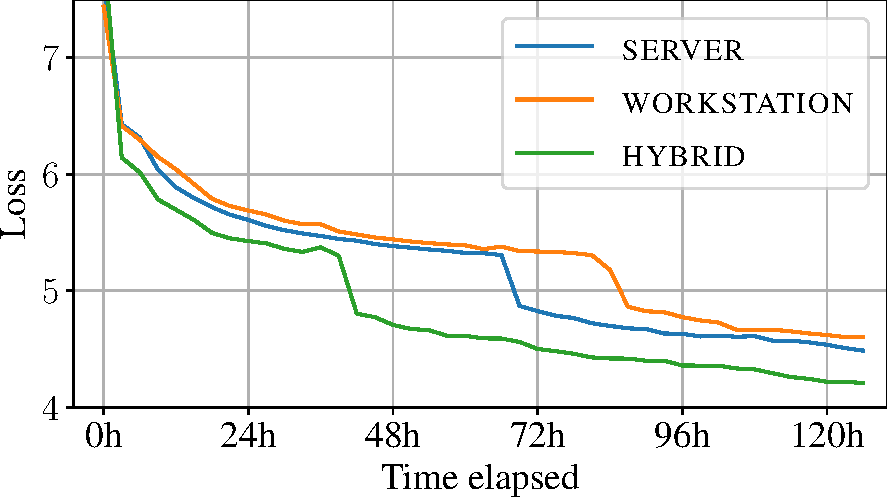
\includegraphics[height=100px]{resources/swav.pdf}
\captionof{figure}{SwAV pretraining performance.}
\label{fig:swav_perf}
\end{minipage}
\begin{minipage}[b][][b]{0.49\textwidth}
\centering
\renewcommand{\arraystretch}{1.2}
\begin{tabular}{lccc}
\toprule
\multicolumn{1}{c}{\multirow{2}{*}{Setup}} & \multicolumn{3}{c}{Algorithm} \\
 & AR & PS & Ours             \\ 
\midrule
A: 8x1Gb/s & \textbf{1.19} & 4.73 & 1.20 \\
B: 16x0.2Gb/s & \textbf{5.3} & 39.6 & \textbf{5.3} \\
C: A + B& 5.69 & 14.1 & \textbf{2.96} \\
D: B + 1x2.5Gb/s & 5.3 & 3.22 & \textbf{3.18} \\
\bottomrule
\end{tabular}
\vspace{8pt}
\captionof{table}{ResNet-50 averaging performance.}
\label{tab:averaging_perf}
\end{minipage}
\vspace{-4pt}

\subsection{Self-supervised pretraining for language understanding}
\label{sect:exp_albert}

Next, we investigate how collaborative training performs for more complex models. In this experiment, we pretrain the ALBERT-large~\cite{albert} masked language model on the WikiText-103 dataset~\cite{wikitext103}. We chose this setup for two reasons: first, ALBERT is very sensitive to the choice of hyperparameters, and specifically batch size, even more than regular Transformers~\cite{trainingtips}. This makes it easier to verify that DeDLOC can reproduce the training conditions of regular data-parallel training. Second, because of weight sharing, training ALBERT is relatively more compute- and less communication-intensive than regular BERT~\cite{bert}, which makes it possible to train with lower bandwidth.
\nocite{paszke2019pytorch}

As before, we follow the exact training configuration from the original paper, but use GPUs instead of TPUs. We use the implementation of ALBERT from the \texttt{transformers} library~\cite{wolf-etal-2020-transformers}. We run all experiments on cloud instances with Tesla T4 GPUs and report the training loss as a function of time, similarly to~\cite{lin2020multinode,switch}. In order to evaluate how DeDLOC performs with different network speeds, we consider the following setups on the same platform with controlled conditions:
\begin{itemize}[leftmargin=*]
   \item \textbf{High-bandwidth:} 16 workers, each with Tesla T4 and 25 Gb/s symmetric bandwidth;
    \item \textbf{Heterogeneous:} same, but with 4x 200 Mb/s, 8x 100 Mb/s and 4x 50 Mb/s bandwidths;
    \item \textbf{Heterogeneous + load balancing:} like Heterogeneous, but with adaptive averaging (Section~\ref{sect:method_algorithm});
    \item \textbf{Auxiliary peers:} the previous setup with 4 additional CPU-only peers at 1 Gb/s bandwidth.
    \item \textbf{Time-varying:} same as previous, but with 8 additional peers at 100 Mb/s. The extra peers are training part-time, jointly alternating between 8 hours of training and 8 hours of downtime.
\end{itemize}
\pagebreak[0]

\begin{minipage}[b][][b]{0.65\textwidth}
\centering
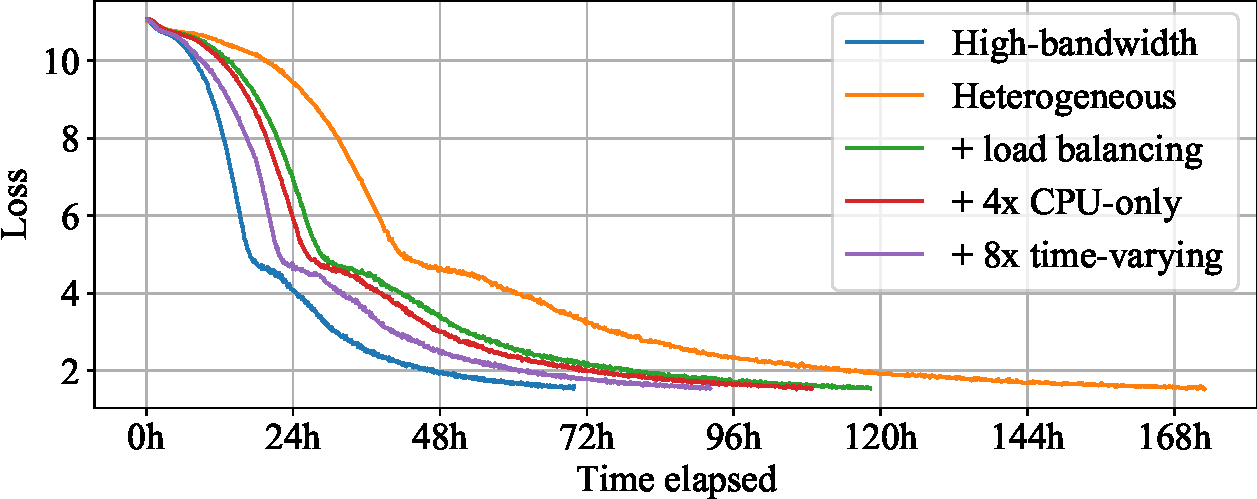
\includegraphics[width=\textwidth]{resources/convergence_albert.pdf}
\vspace{-14pt}
\captionof{figure}{ALBERT pretraining performance.}
\label{fig:albert_perf}
\end{minipage}
\begin{minipage}[b][][b]{0.32\textwidth}
\centering
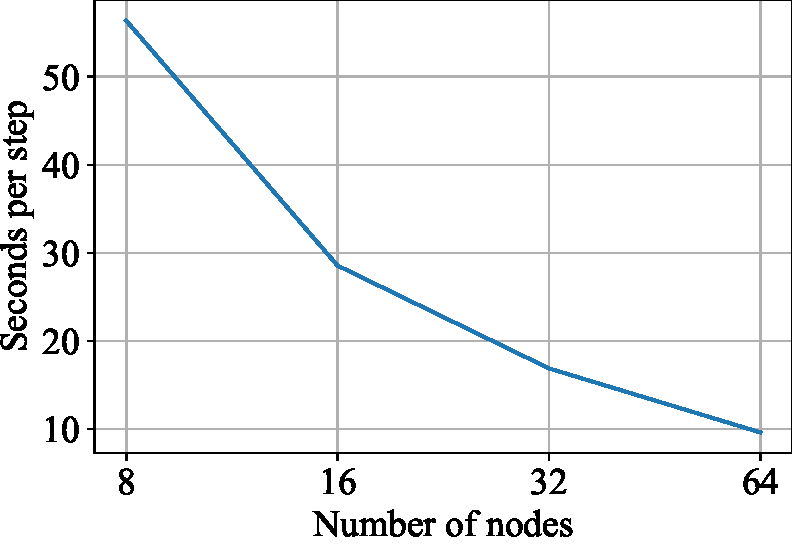
\includegraphics[width=\textwidth]{resources/albert_scalability.pdf}
\vspace{-14pt}
\captionof{figure}{Scalability measurements for ALBERT pretraining.}
\label{fig:albert_scalability}
\end{minipage}

As one can see in Figure~\ref{fig:albert_perf}, naïve training with low-bandwidth peers results in an~$\approx$ 2.5x slowdown compared to high-bandwidth ones. Enabling load balancing accelerates that setup by $\approx47\%$. This effect grows to over 60\% when adding 4 auxiliary peers. Finally, adding 8 part-time peers allows the collaboration to train at 74\% the speed of the high-bandwidth setup without sacrificing the training stability. This turns the latter setup into a viable alternative to traditional distributed training without the need for expensive infrastructure (see the cost analysis in Appendix~\ref{appendix:cost_analysis}). In addition, we demonstrate the high scalability of DeDLOC in Figure~\ref{fig:albert_scalability}, which was obtained by running the same experiment with a varying number of nodes and measuring the time between gradient descent steps. 

\vspace{-6pt}
\subsection{Real-world collaborative training}\label{sect:exp_bengali}
\vspace{-4pt}

For our final evaluation, we organized an actual collaborative training run with volunteer participants, who were asked to pretrain a Transformer masked language model for the Bengali language. This task was chosen deliberately to show the benefits of collaborative training: Bengali has over 230M native speakers who can benefit from recent advances in NLP, but there are few pretrained models available for this language.
We recruited 30 Bengali-speaking volunteers and 10 outside collaborators. All participants received instructions for contributing with free cloud platforms and access to the code for training on local computers. To avoid bias, we did not encourage any specific form of participation: volunteers were free to choose what hardware they contributed and for how long.

Specifically, we trained the ALBERT-large model on Wikipedia and the Bengali part of the OSCAR~\cite{Oscar} multilingual corpus. The model was named sahajBERT after conducting a poll among the participants. We adapted our preprocessing by following the best practices for the Bengali language described in Appendix~\ref{appendix:bn_albert_tokenizer}. To stream from a mix of Wikipedia and OSCAR, the training process iteratively sampled examples from one or the other dataset, as described in Section~\ref{sect:method_system_design}. We accounted for uneven size and quality of data by oversampling Wikipedia by a factor of 2, which resulted in mixing probabilities of 0.23 for Wikipedia and 0.77 for OSCAR. Other hyperparameters were set to the same values as in Section~\ref{sect:exp_albert}. Also, in Appendix~\ref{appendix:xl} we report the results of sahajBERT-XL --- a four times larger model with a specialized architecture that used both GPU and TPU resources.

\begin{figure}[b]
\vspace{-14pt}
% \captionsetup[subfigure]{belowskip=-1pt}
\noindent
\centering
\begin{subfigure}[t]{0.37\textwidth}
\centering
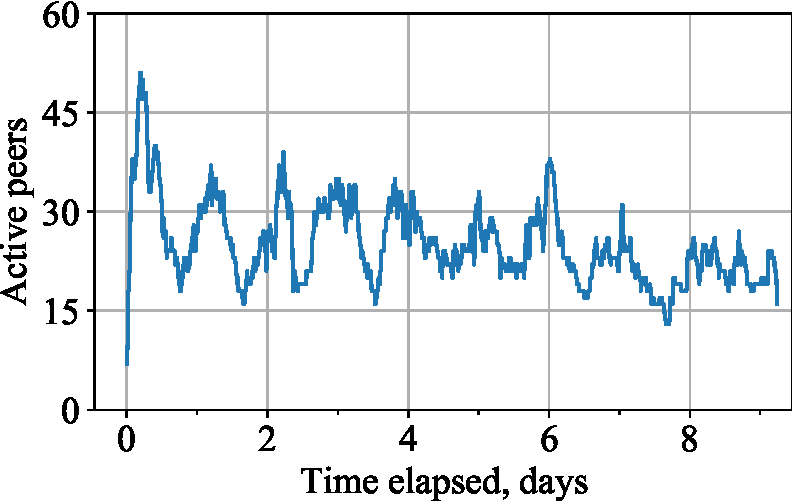
\includegraphics[width=\textwidth]{resources/peer_activity.pdf}
\caption{Collaboration activity.}
\label{fig:activity}
\end{subfigure}
\begin{subfigure}[t]{0.3\textwidth}
\centering
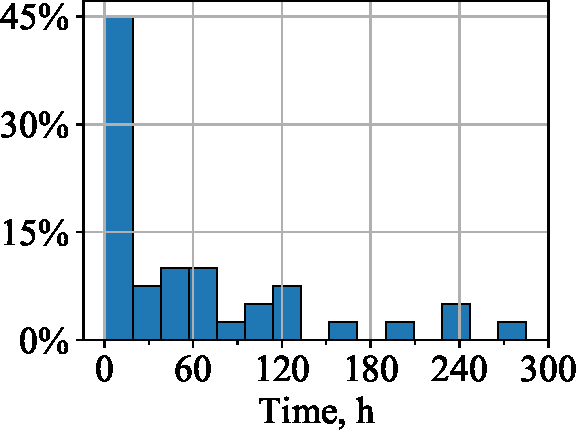
\includegraphics[width=\textwidth]{resources/contrib_hist.pdf}
\caption{Participation time histogram.}
\label{fig:contrib}
\end{subfigure}
\begin{subfigure}[t]{0.3\textwidth}
\centering
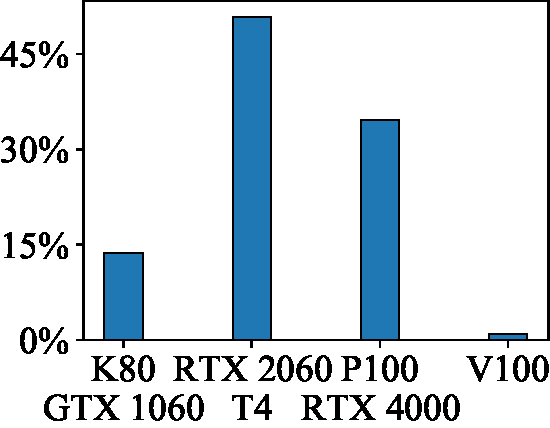
\includegraphics[width=\textwidth]{resources/gpu_hist.pdf}
\caption{Summary of volunteer hardware with example GPUs.}
\label{fig:device}
\end{subfigure}
\vspace{-4pt}
\caption{Collaborative experiment summary.}
\end{figure}


In total, the 40 volunteers contributed compute time from 91 unique devices, most of which were running episodically. Figure~\ref{fig:contrib} shows that although the median GPU time contributed by volunteers across all devices was $\approx$ 1.5 days, some participants ran the training script on several devices, attaining more than 200 hours over the duration of the experiment. With the exception of the start and the end of the collaborative run, the number of simultaneously active devices mostly varied between 15 and 35 depending on the local time. There was less activity in the last 3 days, likely because the volunteers could see that the model has converged on a public Weights \& Biases~\cite{wandb} dashboard.

As depicted in Figure~\ref{fig:device}, individual device performance varied significantly among the collaborators. Along with the resources provided by participants, we also used 16 preemptible single-GPU cloud T4 instances for training.
We have estimated that the average volunteer device consumed 6.95 GB of network traffic per hour of training. While this bandwidth usage is by no means insignificant, it is comparable with cloud gaming~\cite{google_stadia} or high-quality video streaming~\cite{netflix}.

The model converged after 8 days of training, which is 1.8x as fast as regular distributed training with 8 V100 GPUs that we ran as a baseline; Figure~\ref{fig:collab_loss} displays the convergence plots for both setups. At the same time, the stepwise learning curves of the two runs were virtually identical (see Appendix~\ref{appendix:stepwise_learning_curves}), which supports our hypothesis that training with DeDLOC is equivalent to a regular large-batch SGD.
 
\vspace{2pt}
\begin{minipage}[b]{0.49\textwidth}
\centering
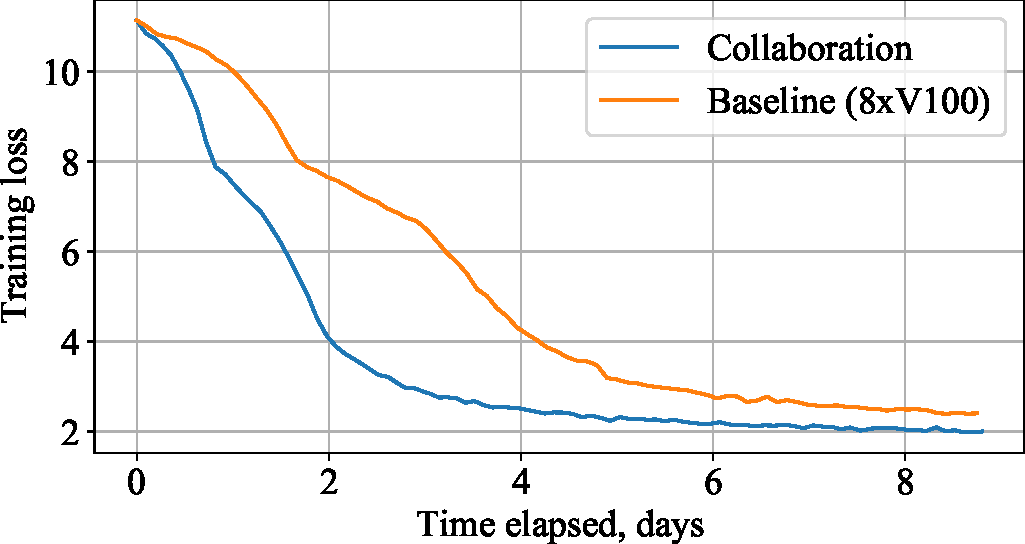
\includegraphics[width=0.95\linewidth]{resources/loss_collab_bengali.pdf}
\vspace{-4pt}
\captionof{figure}{Training progress of sahajBERT.}
\label{fig:collab_loss}
\end{minipage}
\begin{minipage}[b]{0.5\textwidth}
\setlength{\tabcolsep}{2pt}
\renewcommand{\arraystretch}{1.2}
\begin{tabular}{lcc}
\toprule
Model  & Wikiann F1 &NCC Accuracy \\
\midrule
bnRoBERTa           & 82.32 $\pm$ 0.67 &  80.94 $\pm$ 0.45 \\
IndicBERT           & 92.52 $\pm$ 0.45 &  74.46 $\pm$ 1.91 \\
XLM-R               & 96.48 $\pm$ 0.22 &  90.05 $\pm$ 0.38 \\
\midrule
sahajBERT           & 95.45 $\pm$ 0.53 &  91.97 $\pm$ 0.47 \\
sahajBERT-XL        & \bf 96.59 $\pm$ 0.26 & \bf 92.91 $\pm$ 0.43 \\
\bottomrule
\end{tabular}
\captionof{table}{Downstream evaluation results.}
\label{tab:downstream}
\end{minipage}

Finally, we compared the Bengali language representations of sahajBERT with those of other pretrained models on several downstream applications. The first model is XLM-R Large~\cite{xlmr} --- a cross-lingual Transformer-based masked language model that was pretrained on 100 languages and remains a strong baseline for multilingual representation learning. Similarly to sahajBERT, the second model, IndicBERT~\cite{kakwani-etal-2020-indicnlpsuite}, is also based on the ALBERT architecture; however, it was pretrained on 12 languages, including Bengali and Indian English. The third model, bnRoBERTa~\cite{jain2020indictransformers}, is a RoBERTa architecture trained on a monolingual Bengali corpus. We evaluate the model quality on two tasks: WikiANN~\cite{pan-etal-2017-cross} named entity recognition dataset and Soham News Category Classification benchmark from IndicGLUE~\cite{kakwani-etal-2020-indicnlpsuite}. For a detailed description of the setup, refer to Appendix~\ref{appendix:exp_bengali_evaluation}.

As shown in Table~\ref{tab:downstream}, sahajBERT performs comparably to three strong baselines despite being pretrained in a heterogeneous and highly unstable setting.
Notably, our collaboratively trained model outperforms two specialized monolingual baselines and demonstrates competitive results to XLM-R Large, even though the latter has significantly more parameters (560 million instead of 17 million) and was trained on five hundred high-performance data center GPUs instead of tens of low-cost or even free-tier accelerators.
This result confirms previous findings on the benefits of parameter sharing  that were made by authors of ALBERT. Also, it highlights one additional advantage of such architectures: specifically, one can train a high-quality representation model in a communication-constrained setting (for instance, over the Internet) without facing noticeable data transfer bottlenecks.

\section*{Broader Impact}
\label{sect:broader}
\vspace{-4px}

The approach proposed in this work is only a prototype with limited direct consequences, but the long-term goal of training huge models with volunteer computing can have a lasting effect on both the research community and the general public.

\vspace{-6px}
\subsection*{Funding bias vs crowdsourcing bias} 
\vspace{-6px}
The main positive outcome we pursue is to let researchers harness volunteer computing and train models on the scale currently available only to large corporations. Ideally, a deep learning researcher with a promising idea will be able to amass the computation needed to realize this idea by involving volunteers. However, the project's appeal for volunteers depends on many factors such as subject area, current societal trends, and even researcher's personality.

For example, a project about teaching agents to play games~\cite{lc0} or fighting global pandemics~\cite{folding_covid} is likely to attract more resources than deep learning applied to soil science. In essence, volunteer computing is biased towards exciting or socially relevant research the same way as traditional HPC is biased towards the interests of those who fund it.

\vspace{-6px}
\subsection*{Alternative use and misuse} 
\vspace{-6px}
The proposed technology can be used with different economic models. If a deep learning system is immediately useful (e.g. for machine translation, information retrieval, etc), the participants could use it for their needs based on their contributions to training. This can take many forms: several labs combining their hardware and training larger models; a web-service that lets people contribute their compute instead of using ads/subscriptions; or simply a framework that someone can use to run distributed training across two or more datacenters.

Unfortunately, this also allows several opportunities for malicious use. If a machine is hacked, the attacker can use its compute unnoticed by the machine owner --- much the same way that botnets are currently used to mine cryptocurrencies. Furthermore, due to decentalized nature even legitimate Learning@home projects can be hijacked by hackers.

\vspace{-6px}
\subsection*{Security} 
\vspace{-6px}
Using crowdsourced hardware makes Learning@home susceptible to attacks from malicious participants. There are multiple attack vectors already known in P2P community: denial of service attacks, Sybil attacks, Eclipse attacks and more \cite{urdaneta2011survey, sybil_attacks_dht, dos_resistance, sybil_nodes}. Fortunately, there are variations of the DHT protocol that make it resistant to said attacks: if a reader wishes to learn more about DHT security, we recommend starting with \cite{urdaneta2011survey}.

Another source of vulnerability stems from the sequential nature of neural networks. If a single expert were to return incorrect (e.g. NaN) outputs or gradients, it could compromise the outputs of the entire network and even poison adjacent nodes through backpropagation. Recent studies expose similar attack patterns on federated learning systems \cite{bagdasaryan2018backdoor, bhagoji2018analyzing}.

The redundant nature of mixture-of-experts layers provides some degree of resistance against those attacks. A single malicious expert will only affect a small fraction of inputs that pass through this specific expert. Furthermore, a trainer with access to predictions from multiple experts could provide a higher degree of robustness by using statistical techniques (e.g., by ignoring outlier gradients). However, such techniques need to be carefully designed so as not to introduce harmful side effects.

\vspace{-6px}
\subsection*{The burden on the network} 
\vspace{-6px}
Finally, we would like to point out the potential harm that our approach can do to network infrastructure. The experiments we ran in Section \ref{sect:exp_throughput} saturate with the bandwidth of $100-200$Mbps, most of which is tensors passed between experts and trainers. 

This coincides with the typical home internet speed available in major cities of developed countries. However, not all ISPs design their infrastructure for users who always use up all their bandwidth. If too many Learning@home participants are located in one LAN or MAN, it can cause congestion or even failures in the network infrastructure. 

Similar situations frequently took place in late 2000s due to growing popularity of BitTorrent for file sharing. Fortunately, the network infrastructure is continually improving, which leads us to believe that this problem will eventually be solved. Until then, we describe several ways to reduce network load of Learning@home in Appendix E.




\section*{Acknowledgements}
We thank Stas Bekman, Dmitry Abulkhanov, Roman Zhytar, Alexander Ploshkin, Vsevolod Plokhotnyuk and Roman Kail for their invaluable help with building the training infrastructure.
Also, we thank Abhishek Thakur for helping with downstream evaluation and Tanmoy Sarkar with Omar Sanseviero, who helped us organize the collaborative experiment and gave regular status updates to the participants over the course of the training run.
Finally, we thank the anonymous reviewers for their feedback on the content and the presentation of our paper.

In addition, authors would like to thank the students of Yandex School of Data Analysis who volunteered to participate in preliminary experiments.

We kindly thank all participants of the Neuropark community\footnote{\href{https://huggingface.co/neuropark}{huggingface.co/neuropark}} who contributed to sahajBERT training. Below, we list the community members who agreed to provide their name for this paper: Aakash Gupta, Aninda Goswamy, Anjali Prasad, Anurag Singh, Arijit Sarkar, Chirranjit Ghosh, Debajit Mallick, Ibraheem Muhammad Moosa, Ishan Bagchi, Khalid Saifullah, Laxya Agarwal, Manan Dey, Mir Ali, Mrinal Mathur, Nilavya Das, Preetha Suri, Priyadarshan Sarkar, Sagnik Roy, Sahil Saha, Sanjeev Kumar, Sanskar Upadhyay, Shyam Sunder Kumar, Soumi Kaibartya, Subhranil Sarkar, Sujit Pal, Syed Modassir Ali, Tanmoy Sarkar, and Vaishali Pal.

Training sahajBERT-XL and hybrid GPU-TPU experiments were made possible by John Kintree, Debajit Mallick, Avijit Saha, Ishan Bagchi, Nilavya Das, Priyadarshan Sarkar, Sagnik Roy, Eduard Pokonechnyy, Arina Ruck. Finally, we would like to acknowledge Tanmoy Sarkar for setting up the backbone peer for sahajBERT-XL on his server and contributing to the evaluation codebase.


The computational resources for internal experiments on cloud instances were provided by the Amazon Research Awards program.

\bibliographystyle{unsrt}
\bibliography{bibliography}

\clearpage
\section*{Contributions}
\label{sec:contributions}

\vspace{-2pt}
\subsection*{Conceptual}

\textbf{Michael Diskin} derived the optimization problem for adaptive averaging.

\textbf{Max Ryabinin} designed and led the research.

\textbf{Thomas Wolf} initially proposed to run collaborative training with the community participants.

\textbf{Gennady Pekhimenko} supervised the work from the systems design point of view.

\vspace{-2pt}
\subsection*{Technical}

\textbf{Alexey Bukhtiyarov} implemented the core large-batch decentralized optimization procedure. 

\textbf{Dmitry Popov} implemented the support of client mode and auxiliary CPU peers for training.

\textbf{Michael Diskin} implemented and conducted the ALBERT pretraining experiments.

\textbf{Anton Sinitsin and Dmitry Pyrkin} implemented and conducted the SwAV pretraining experiments.

\textbf{Quentin Lhoest} designed and implemented the training data streaming logic.

\textbf{Alexander Borzunov and Lucile Saulnier} proposed and implemented the authentication protocol.

\textbf{Max Ryabinin} provided the initial code for cloud-based ALBERT pretraining.

\textbf{Maxim Kashirin, Denis Mazur, and Ilia Kobelev} implemented the libp2p integration.

\textbf{Max Ryabinin} supervised the development of the project and reviewed the code of contributions.

\vspace{-2pt}
\subsection*{sahajBERT}

\textbf{Michael Diskin, Alexey Bukhtiyarov, and Dmitry Popov} created the notebooks with instructions.

\textbf{Lucile Saulnier} built the tokenizer for sahajBERT and implemented Bengali-specific preprocessing.

\textbf{Michael Diskin, Lucile Saulnier, Max Ryabinin, and Alexander Borzunov} managed the running sahajBERT experiment, monitored its performance, answered the questions of participants, and investigated the occurring errors.

\textbf{Albert Villanova del Moral} implemented and conducted downstream finetuning experiments.

\textbf{Michael Diskin} created the dashboards and implemented continuous reporting of experiment metrics.

\textbf{Alexey Bukhtiyarov} added automatic model state fetching and pushing to Model Hub.

\textbf{Yacine Jernite} helped to find the Neuropark community that was interested in collaborative training. 

\vspace{-2pt}
\subsection*{Writing}

\textbf{Max Ryabinin} composed the initial structure of the paper, wrote its abstract and the introduction.

\textbf{Max Ryabinin, Dmitry Popov, and Alexey Bukhtiyarov} discussed the distributed training, volunteer computing, and federated learning aspects of related work, respectively.

\textbf{Max Ryabinin, Lucile Saulnier, and Yacine Jernite} wrote the conclusion of the work.

\textbf{Michael Diskin} discussed the use of group-based All-Reduce for training in larger collaborations.

\textbf{Michael Diskin} conducted the cost analysis of different distributed training approaches.

\textbf{Maxim Kashirin, Denis Mazur, and Ilia Kobelev} described methods for NAT traversal along with peer-to-peer networking.

\textbf{Max Ryabinin, Michael Diskin, and Anton Sinitsin} outlined decentralized data streaming.

\textbf{Yacine Jernite} assessed the environmental implications of DeDLOC.

\textbf{Gennady Pekhimenko and Thomas Wolf} helped improve the general presentation of the work.

\textbf{Max Ryabinin, Michael Diskin, and Gennady Pekhimenko} edited the final version of the paper.
\clearpage

\appendix
\section*{Supplementary Material}

\section{Federated learning}
\label{appendix:related_federated}

Federated learning (FL) is an approach that trains the model on decentralized data stored on many devices without sharing private training data~\cite{FedLearningOriginal}. This scenario is currently gaining more popularity with the rising awareness of data privacy and emerging legal constraints, such as GDPR. Similarly to our setting, FL systems must deal with unreliable heterogeneous hardware. However, their main goal is to ensure the data privacy, which often leads to sacrifices in terms of efficiency.

Most practical FL systems utilize a central parameter server that aggregates local gradients from workers and updates the global model.
As we increase the number of workers, the total system performance becomes bounded by the throughput of this server.
The problem is exacerbated by secure aggregation protocols~\cite{PracticalSecureAggregation, FedLearningDiffPrivacy} that further increase the communication overhead to ensure data privacy.
To account for these limitations, production FL systems perform each update using only a small random subset of peers, while the rest remain idle~\cite{FedLearningAtScale}. Contrary to this, our goal is to maximize the training performance by running computations on all peers.

Another recent line of work explores federated learning algorithms with a decentralized communication topology. %~\cite{TODO}.
Maintaining data privacy in these conditions also requires specialized techniques that introduce communication overhead. For instance, \cite{FedLearningDecentralized} proposes a system where workers cannot share parameters directly, relying on a secure peer-to-peer knowledge distillation instead. %even don't transmit model parameters and perform training via global knowledge distillation.

% In order to maintain security in , these algorithms also adopt privacy protection techniques at a significant cost of utility~\cite{FedLearningAdvancesProblems} 
% The alternative approach is decentralized FL, where no central server is required. These methods should . Some architectures even don't transmit model parameters and perform training via global knowledge distillation~\cite{FedLearningDecentralized}. No practical FL system has successfully used this paradigm and it is still an open research problem.

The above discussion makes it clear that the purpose of the federated learning is orthogonal to ours: we aim to train the global model on publicly available data and achieve the best possible performance.


% \begin{itemize}
%     \item what is it trying to achieve and why
%     \item clearly explain how we are different from federated learning
%     \item they care about data privacy (at a cost of compute/network overhead), we care about training samples/s on public data
%     \item practical FL systems require PS or similar architectures, hard to scale
% \end{itemize}

\section{Optimal averaging strategy via linear programming}
\label{appendix:lp_optimization}
Recall that DeDLOC finds the optimal communication strategy by solving the following problem:

\begin{equation}
\label{eq:main_problem_appendix}
\begin{array}{rclll}
\underset{a, g, c}{\max} & &
                                \min\Bigg(\frac{\sum_{i=1}^n s_i \cdot c_i }{B},\ 
                                     \frac{ \min_i\sum_{j} g_{j i}}{P}\Bigg)&\quad&\\
\textrm{s.t. } &\quad & g_{i j} \leq \min_{k: c_k{=}1} a_{k i}  &\quad&\forall i, j \\
                 & \quad  & \sum_{j \neq i}\left( a_{j i} + g_{j i}\right) \leq d_{i} & \quad&\forall i \\
                 & \quad &   \sum_{j \neq i}\left( a_{i j} + g_{i j}\right) \leq u_{i} & \quad&\forall i \\
                 & \quad &   a_{i j} + g_{i j} \leq t_{i j} & \quad&\forall i, j \\
                 & \quad &   a_{i j} \geq 0 \And g_{i j} \geq 0 \And c_i. \in \{0, 1\}& \quad&\forall i, j \\
\end{array}
\end{equation}
Here, $a_{ij}$ denotes the fraction of network throughput allocated to sending gradients from peer $i$ to peer $j$ for aggregation, $g_{ji}$ is the corresponding fraction for returning the averaged tensors back to sender, and $c_i$ is a binary indicator that represents whether or not peer $i$ computes gradients. The remaining variables are parameters that denote peer compute performance $s_i$, maximum download and upload speeds ($d_i$ and $u_i$ respectively) and regional limitations of peer-to-peer throughput ($t_ij$). Finally, $B$ denotes the global target batch size per step and $P$ is the number of model parameters.

As stated earlier in Section~\ref{sect:method_algorithm}, the DeDLOC peers need to find the optimal strategy during each averaging round. As such, we must ensure that the procedure for solving~\eqref{eq:main_problem_appendix} does not introduce any significant overhead. To that end, we reformulate the problem as a linear program by means of several consecutive reductions, which are described below.

\paragraph{Max-min LP reduction.} First, we replace the original max-min objective with a linear one by following the technique described in~\cite{kaplan1974application}: we maximize a new surrogate variable $\xi$ and replace the inner $\min$ by two additional constraints:

\begin{equation}
\label{eq:main_problem_appendix_minmax}
\begin{array}{rclll}
\underset{a, g, c}{\max} & & \xi &\quad&\\
\textrm{s.t. }  &\quad& \xi \leq \frac{\sum_{i=1}^n s_i \cdot c_i }{B} & & \\
                 &\quad & \xi \leq \frac{ \sum_{j} g_{j i}}{P}  &\quad&\forall i \\
                %  &\quad & g_{i j} \leq \min_{k: c_k{=}1} a_{k i}  &\quad&\forall i, j \\
                %  & \quad  & \sum_{j \neq i}\left( a_{j i} + g_{j i}\right) \leq d_{i} & \quad&\forall i \\
                %  & \quad &   \sum_{j \neq i}\left( a_{i j} + g_{i j}\right) \leq u_{i} & \quad&\forall i \\
                %  & \quad &   a_{i j} + g_{i j} \leq t_{i j} & \quad&\forall i, j \\
                %  & \quad &   a_{i j} \geq 0 \And g_{i j} \geq 0 \And c_i \in \{0, 1\}& \quad&\forall i, j \\
\end{array}
\end{equation}


\paragraph{Binary to LP relaxation.} Second, we must account for the binary variable $c_i$. From a formal perspective, using these indicators transforms our problem into a binary mixed-integer program with a combinatorial worst-case complexity. However, for this specific problem, it is possible to rewrite the constraints in such a way that $c_i$ can be treated as a continuous variable $0\leq c_i\leq 1$:%\nocite{lp_relaxation_largescale}
\begin{equation}
\label{eq:appendix_c_relax}
\forall i, j, k \in 1\dots n \quad g_{ij} \leq a_{ki} + (1 - c_k) \cdot d_i
\end{equation}

For $c_k = 1$, the above equation~\eqref{eq:appendix_c_relax} is exactly equivalent to the original constraint $g_{i j} \leq \min_{k: c_k{=}1} a_{k i}$. In turn, setting $c_k < 1$ for some $k$ effectively removes the corresponding peer $k$ from the $\min$ operator, allowing participant $i$ to aggregate tensors with up to its maximum download speed $d_i$ instead of waiting for peer $k$. The $d_i$ factor in~\eqref{eq:appendix_c_relax} can be replaced with any large positive number as long as the constraint~\eqref{eq:appendix_c_relax} is not saturated for $c_k{=}0$. In practice, $c_k \neq 1$ corresponds to peer $k$ \textbf{not} computing gradients, but still assisting in gradient aggregation.

Applying the two above reductions, we get the following linear program:

\begin{equation}
\label{eq:main_problem_appendix_relaxed}
\begin{array}{rclll}
\underset{a, g, c}{\max} & & \xi &\quad&\\
\textrm{s.t. }  &\quad& \xi \leq \sum_{i=1}^n s_i \cdot c_i\; / \;B & & \\
                 &\quad & \xi \leq \sum_{j} g_{j i}\; / \;P  &\quad&\forall i  \\
                 &\quad & g_{ij} \leq a_{ki} + (1 - c_k) \cdot d_i  &\quad&\forall i, j, k \\
                 & \quad  & \sum_{j \neq i}\left( a_{j i} + g_{j i}\right) \leq d_{i} & \quad&\forall i \\
                 & \quad &   \sum_{j \neq i}\left( a_{i j} + g_{i j}\right) \leq u_{i} & \quad&\forall i \\
                 & \quad &   a_{i j} + g_{i j} \leq t_{i j} & \quad&\forall i, j \\
                 & \quad &   a_{i j} \geq 0& \quad&\forall i, j \\
                 & \quad &   g_{i j} \geq 0& \quad&\forall i, j \\
                 & \quad &  0 \leq c_i \leq 1 & \quad&\forall i \\
\end{array}
\end{equation}

To avoid additional synchronization steps, each peer within DeDLOC solves the above problem~\eqref{eq:main_problem_appendix_relaxed} independently using the interior point solver~\cite{andersen}. Based on the obtained solution, peer $i$ will aggregate a fraction of gradients proportional to its effective throughput: 
\begin{equation}
\text{fraction}_i \propto \frac{\min_j g_{ij}}{ \sum_k \min_j g_{kj}}.
\end{equation}
Furthermore, if $c_i\neq1$, the corresponding participant will disregard its local gradients. In the future, it may be possible to allow such peers to contribute partial gradients akin to~\cite{deepgradientcompression}. However, we leave this investigation to future work.

For certain collaboration compositions, there can be multiple optimal strategies with equal training throughputs. To ensure that all participants act according to the same strategy, we require each peer to solve~\eqref{eq:main_problem_appendix_relaxed} using a deterministic interior point algorithm with globally consistent hyperparameters~\cite{scipy}.

Another practical consideration is that some peers are unable to compute gradients or perform aggregation (for instance, due to networking issues described in Section~\ref{sect:method_system_design}). To account for these limitations, we exclude such peers from aggregation in $\frac{\sum_{i=1}^n s_i \cdot c_i }{B}$ and $\frac{\sum_{j} g_{j i}}{P}$ terms for compute and network resources, respectively.

\section{Fault tolerance}\label{appendix:groups}

In practice, using DeDLOC with large collaborations will eventually require dealing with node failures. If the failures are rare, it is possible to restart the failed steps until they succeed. However, if the collaboration size increases, this strategy will eventually become impractical.

One possible solution is to replace the global (collaboration-wide) All-Reduce with several parallel operations, which is known as Group All-Reduce~\cite{wagma} or Moshpit All-Reduce~\cite{moshpit}. Each operation involves a small independent group of $m$ peers, whereas the groups themselves are formed in such a way that the collaboration can obtain the global average in a logarithmic number of rounds.

Under this strategy, any failed device will only affect its local group instead of the entire collaboration. Furthermore, each individual group will have a higher success rate, since it contains $m\ll n$ peers. In turn, the drawback of using group-based All-Reduce is that the collaboration will need $\lceil\log_m n\rceil$ steps to obtain the global average.

We can select the optimal group size by minimizing the \textit{expected} number of iterations required to compute the global average, including both restarts from node failures and the overhead from using Group All-Reduce. For reference, we include the optimal group sizes for typical collaborations and failure rates in Figure~\ref{fig:optimal_m}. In all our experiments, the optimal group size was $m{=}n$ due to a small number of participants and very rare significant network failures.

\begin{figure}
    \centering
    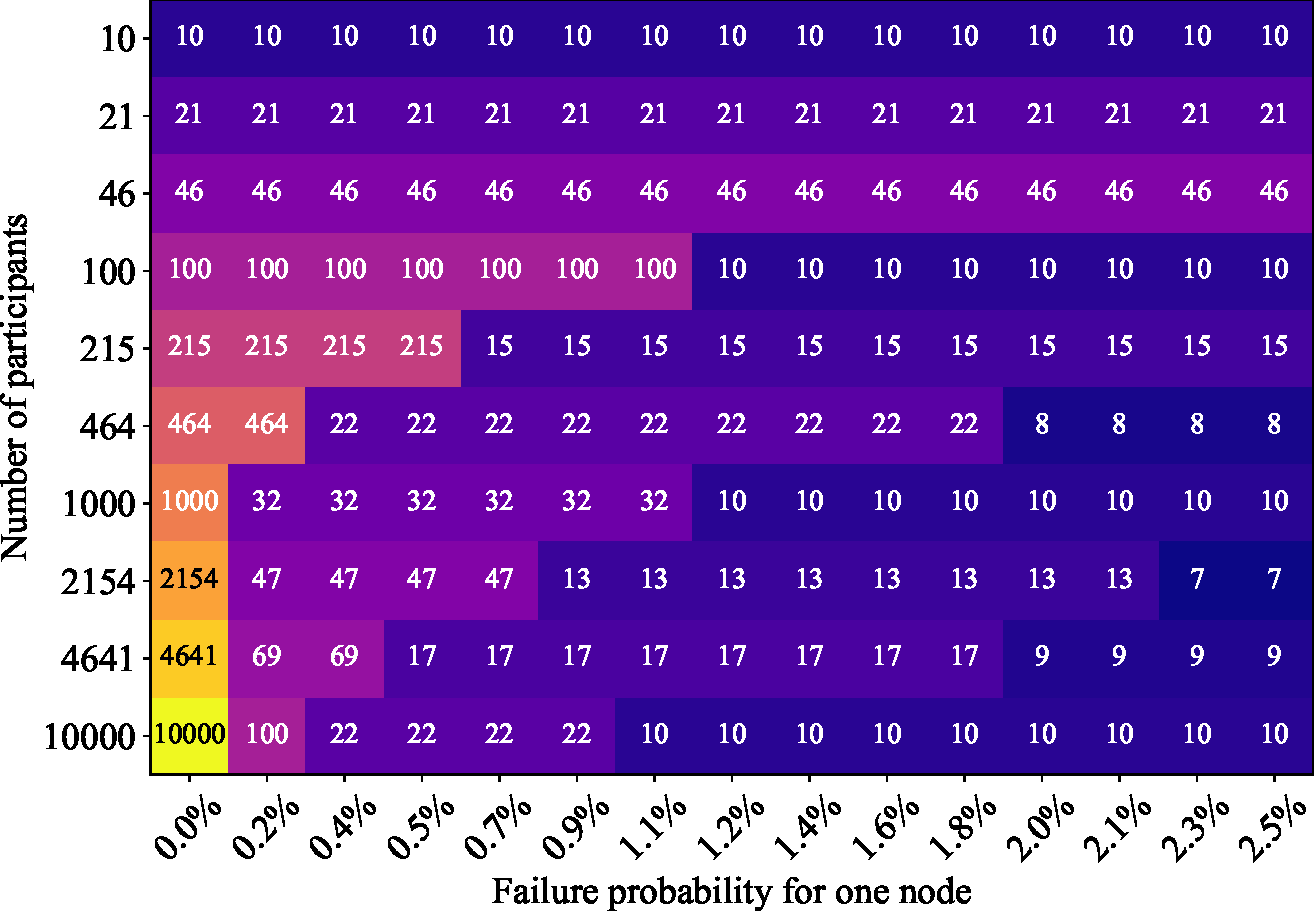
\includegraphics[width=0.95\linewidth]{resources/optimal_group_size.pdf}
    \caption{Optimal group size for different collaboration sizes and failure rates.}
    \label{fig:optimal_m}
    \vspace{-16pt}
\end{figure}


\section{Network address translation}\label{appendix:nat_firewall}

Collaborative training, similarly to any other application incorporating peer-to-peer communication, is susceptible to a number of networking issues, among which the most common is the inability to accept incoming connections due to Network Address Translation, or NAT~\cite{Biggadike05natblaster:establishing}. The primary function of NAT is to separate the address space of the local network from the global address space by dynamically translating addresses and port numbers of outgoing sessions into public endpoints. Therefore, NAT helps deter the rapid depletion of IPv4 addresses and provides additional security by hiding the local network structure from external parties. However, this also means that NAT devices only authorize outgoing connections, since the dynamic mapping of local endpoints makes it impossible to forward incoming packets to the proper internal host.

For the purposes of the current work, NAT devices can be categorized into two groups --- cone and symmetric. A cone NAT translates an internal IP address and port to the same globally routable endpoint regardless of the destination host, whereas a symmetric NAT allocates different address mapping for each destination host. In case of UDP traffic, the cone NAT can be traversed using the mechanism of UDP Hole Punching. Briefly put, this technique consists of two stages. During the first phase, peers A and B connect to the same globally accessible rendezvous server using the STUN protocol~\cite{STUN}  and exchange their public and private endpoints. The rendezvous server is often called the STUN server by the name of the protocol. At the next step, both peers start sending UDP data packets to each other's endpoints. If A's packet reaches NAT B before B's packet ``punches a hole'', then it is dropped by the NAT B, but when the B's packet reaches NAT A shortly after this, the outgoing session has already been initiated by A, so the B's request is successfully forwarded to A. If both peers happen to ``punch a hole'' in their NATs before the arrival of the counterpart's packet, then the connection is established immediately.

For the TCP traffic, hole punching is also possible, though it has to overcome additional API issues that arise because of the client-server paradigm around which TCP was designed. However, peer-to-peer communication over TCP connections is more robust than over UDP, since NAT usually timeouts the UDP port mapping, thus periodical keep-alive messages must be transmitted. As reported in~\cite{hole_punching}, currently almost two thirds of all NAT vendors provide devices which are compatible with TCP hole punching, that is, consistently map private endpoints and do not send back Reset packets to unsolicited requests.

As for the symmetric NAT, only relaying through a third-party proxy can help establish the connection between peers. This is supported with the TURN protocol~\cite{TURN}. If two peers fail to connect via hole punching, they appeal to the TURN server for an interaction through it.

% Firewall is another obstacle for peer-to-peer networks. It is a system that controls and filters network traffic due to given rules. Each rule can restrict or allow connections. The main goal of a firewall is to protect subnetworks and dedicated hosts from attacks and unauthorized access. 

% Firewalls can be configured with quite strict rulesets. According to the specified rules, connections can be established only by allowlists, or incoming restrictions can be restricted at all. Such settings can lead to the unavailability of the host in peer-to-peer networks.

\section{Peer-to-peer network infrastructure}\label{appendix:p2p}

To enable peer-to-peer interactions that can bypass NAT, we can use the libp2p framework~\cite{libp2p}. Each peer has a set of multiaddresses that allow other participants to establish a connection. Multiaddress comprises an IP address, an L4 protocol (TCP/UDP) with a port, an optional high-level protocol (QUIC), and a peer identifier. A peer can listen to several transport protocols, but it may have only one identifier.

After peers connect to the network, they can interact with each other via their respective identifiers. There are no dedicated STUN and TURN servers in the libp2p network: their role is played by public participants. The network must contain at least 4 publicly accessible peers to be able to recognize public addresses of newly connected peers. Optimally, these are well-known peers with multiaddresses known to all participants. Upon joining, a new node synchronizes with the DHT used for routing and receives information about other available peers. After that, a peer can interact with other participants using their peer id. If the network can get the public address of the peer, then other participants will be able to connect to it.

If a public address of the peer is not available or two peers are using different transport, the communication can be started by relaying requests via an intermediate participant.
Libp2p supports the autorelay feature that allows finding the best relay automatically. When autorelay is enabled, a public peer can serve as a relay for other participants, and a private peer will find the best relay.

\vspace{-2pt}
\section{Cost analysis}\label{appendix:cost_analysis}

In this section, we provide a detailed cost analysis of several hardware and networking setups that can be used for both tasks described in Section~\ref{sect:experiments}, namely, SwAV and ALBERT pretraining.

For simplicity, we only consider temporary resource ownership, i.e., renting GPU-enabled servers instead of building it on-premise. The latter option can be more cost-efficient in the long term, but might be impractical if only a few training runs are required. For the same reason, we do not consider discounts available for committed usage of the same resource over multiple years. As for the rented resources, there are several general hardware categories that we consider:

\begin{enumerate}[leftmargin=*]
    \item High-performance cloud GPU --- dedicated instances with multiple high-end compute accelerators and extremely fast device interconnect.
    \item Low-end cloud GPU --- single-GPU instances with NVIDIA M60, T4 or P40, linked with a fast (preferably intra-datacenter) network of 10--50 Gb/s.
    \item Commodity GPUs --- regular desktop-like machines with consumer-grade GPUs, like NVIDIA RTX 2070, 2080 Ti, 3070. On average, they can have higher performance than low-end cloud devices, but lower network throughput (50--200 Mb/s).
    \item Volunteer hardware --- almost the same class of devices as in the previous section, with the same advantages and disadvantages, but ``free'' for the experiment organizers.
\end{enumerate}

For a fair comparison, we consider three types of GPU instances: cloud V100, cloud T4 and commodity GPUs from peer-to-peer marketplaces, such as \url{vast.ai} or \url{golem.ai}. While several cloud providers offer newer generation GPUs (NVIDIA Ampere), this GPU lineup is still in an active rollout phase, which causes significant price fluctuations. Thus, we base our conclusions on more established generations of GPUs. 

In addition to GPU instances, DeDLOC can also benefit from non-GPU servers that act as auxiliary parameter aggregators. The only real requirement for such servers is high network bandwidth. As such, we consider additional resource types:
\begin{enumerate}[leftmargin=*]
    \item Premium cloud VMs --- low-end instances from premium cloud providers. We consider instances with 2 cores, 16GB RAM and 25 Gb/s maximum bandwidth (symmetric).
    \item Economy cloud VMs --- similar cloud instances (or dedicated servers) from economy cloud providers. For this run, we consider instances with the same 2 cores / 16GB RAM, but only 300--1000 Mb/s symmetric bandwidth (depending on the provider).
    \item Volunteer non-GPU devices --- in theory, it is possible to run collaborative training entirely on volunteer devices with zero hardware expenses for the organizer. However, we omit this option as it trivializes our cost analysis.
\end{enumerate}

On top of that, all cloud and marketplace instances can be rented in a guaranteed (``on-demand'') or a non-guaranteed option. In the latter scenario, the resources are offered at a significant discount, but the resource provider can terminate such instances at any time.

Based on the available resource types and ownership models, we assemble six server fleets with approximately equal training performance in our two experimental setups. For convenience, we order these setups by how difficult they are to operate (easiest-first):

\begin{itemize}[leftmargin=*]
    \item Single high-end node --- 8 x NVIDIA Tesla V100: easiest to operate, but the most expensive option.
    \item Preemptible high-end node has the same hardware but costs less due to irregular availability, which creates a need for regularly saved checkpoints.
    \item Distributed nodes --- 16 x NVIDIA Tesla T4: homogeneous, require distributed optimization.
    \item Distributed + preemptible --- same but preemptible, can be used with a framework that supports elastic training, such as TorchElastic\cite{pytorch_elastic} or Elastic Horovod\cite{elastic_horovod}.
    \item Distributed + heterogeneous --- 5x NVIDIA GTX 1080 Ti, 3x RTX 2070, 1x 2070S, 2x 2080, 4x 2080 Ti, 1x 3070. This configuration has lower bandwidth, thus additional CPU-only peers are needed for efficient averaging.
    \item Collaborative training --- for this setup, we assume that the GPUs from the previous setup are available from volunteers. In that case, the only sources of expenses for the organizer are networking and CPU-only nodes.
    
\end{itemize}

As one can see in Table~\ref{tab:cost}, using a single high-end node is the most expensive alternative. Switching to multiple lower-end nodes and using non-guaranteed instances reduces the cost by a factor of $\approx3$x each. Finally, the volunteer infrastructure is two orders of magnitude cheaper than the high-performance setup. However, some of this price difference is effectively shifted to volunteers. Based on average electricity and networking costs of household Internet connections, we estimate the expense at \$9--30 \textit{per volunteer per month}, assuming 16 volunteers with equivalent GPUs. However, actual costs can vary based on the region, time duration and the exact hardware used by each volunteer.

\begin{table}[b]
\vspace{-14pt}
\renewcommand{\arraystretch}{1.1}
\centering
\caption{Costs of training setups.}
\vspace{6pt}
\label{tab:cost}
\begin{tabular}{@{}lcc@{}}
\toprule
Setup & Instance types & Monthly cost \\ \midrule 
\multirow{2}{*}{Cloud on-demand} & 8xV100 & \$16,898 \\
 & 16xT4 & \$5,299 \\ 
\multirow{2}{*}{Cloud preemptible} & 8xV100 & \$5,133 \\
 & 16xT4 & \$2,074 \\
Marketplace & 4xCPU+16xGPU & \$5,148 \\ 
Volunteer & 4xCPU & \$257 \\ \bottomrule
\end{tabular}
\end{table}

Finally, we want to reiterate that the above setups require different amounts of effort (and expertise). Training on a single high-end node can be done with virtually no code changes in major deep learning frameworks, such as TensorFlow~\cite{tensorflow2015-whitepaper} or PyTorch~\cite{paszke2019pytorch}. In contrast, multi-node (and especially elastic) setups require specialized distributed training frameworks and careful performance tuning. Finally, working with volunteer or marketplace instances introduces a new layer of complexity, which is addressed in this paper.

\paragraph{Networking costs.} When done naïvely, training with geographically distributed participants can incur significant networking expenses. For instance, when using preemptible cloud GPUs from a major provider, allocating these GPUs in different regions can incur additional costs of more than \$3000 per month, compared to a total hardware cost of \$2074 for the same period.

More importantly, using premium non-GPU instances for collaborative training will also incur additional networking costs. Based on our preliminary experiments, a collaborative training setup equivalent to Table~\ref{tab:cost} would lead to an average networking bill of \$5000-6000 per month.
Fortunately, it is possible to circumvent this expense by using cloud providers that do not charge additional costs for network traffic. These providers typically offer less reliable instances with lower maximum bandwidth, which is not a significant issue for DeDLOC.

As a general recipe for reproducing our experiments, we recommend using one of the two setups. When running experiments internally, one can use any major cloud provider as long as all instances are \textit{configured to avoid cross-regional networking costs} (e.g. use internal address space).
In contrast, when training with actual volunteer devices, we recommend using cloud providers without additional networking charges or existing server infrastructure.

\section{Convergence analysis}
\label{appendix:convergence_analysis}
As discussed in Section~\ref{sect:method_general}, DeDLOC updates parameters only after accumulating the gradients for the target number of samples from up-to-date peers. However, due to network-related delays, peers can process more samples than required in some cases. Thus, we can analyze DeDLOC as a regular SGD with varying batch sizes, which allows us to adapt the existing convergence bounds from the optimization literature. More formally, consider a standard optimization problem

\begin{equation}
    \min_{x\in\mathbb{R}^n} f(x),
\end{equation}

which is solved by SGD. We denote the gradients for step $k$ as $\mathbb{E}[g^k|x^k]=\nabla f(x^k)$ and the corresponding update as $x^{k+1}=x^k-\gamma_k g^k$.

Denote the variance of a single stochastic gradient as $\mathbb{E}\left[\left(\nabla f(x^k,\xi_i^k)-\nabla f(x^k)\right)^2|x^k\right]\leq \sigma_0^2$ and the target batch size as $m$. At step $k$, DeDLOC will accumulate gradients from $m_k\geq m$ samples:

\begin{equation}
    g^k=\frac{1}{m_k}\sum_{i=1}^{m_k}\nabla f(x^k,\xi_i^k).
\end{equation}

Thus, the gradient averaged over a minibatch of $m_k$ i.i.d. samples will have the following variance:

\begin{equation}
    \mathbb{E}\left[\left(g^k-\nabla f(x^k)\right)^2| x^k\right]=\frac{1}{m_k^2}\sum_{i=1}^{m_k}\mathbb{E}\left[\left(\nabla f(x^k,\xi_i^k)-\nabla f(x^k)\right)^2| x^k\right]\leq \frac{1}{m_k^2}\sum_{i=1}^{m_k}\sigma_0^2.
\end{equation}

Because $m_k\geq m$,

\begin{equation}
    \frac{1}{m_k^2}\sum_{i=1}^{m_k}\sigma_0^2=\frac{\sigma_0^2}{m_k}\leq\frac{\sigma_0^2}{m},
\end{equation}

which allows us to reuse the existing SGD convergence bounds from the optimization literature~\cite{stich2019unified,khaled2020unified}. For instance, we can use Theorem 5 from~\cite{stich2019unified} and plug in $\frac{\sigma_0^2}{m}$ as gradient variance (with notation also from~\cite{stich2019unified}), getting the following result: 

\begin{equation}
    \mathbb{E}{ f(\bar x_T) - f^\star} + \mu \mathbb{E}{|x_{T+1}-x^\star}|^2 \leq \min \left\{ 64 L R^2 \exp \left[-\frac{\mu T}{4L} \right] + \frac{36 \sigma_0^2}{\mu m T} ,  \frac{2LR^2}{T} + \frac{2 \sigma_0 R}{\sqrt{mT}}  \right\}.
\end{equation}

\section{Decentralized data streaming}
\label{appendix:decentralized_dataset_streaming}
In this section, we propose a generalization of our data streaming approach described in Section~\ref{sect:method_system_design} to a setting without any central data storage. Namely, we offer a way to 
to distribute large datasets across all participants by sharding the examples in the same manner that was used previously.

Specifically, this approach is based on the notion of a local buffer combined with the decentralized metadata storage enabled by the DHT. When a peer joins the experiment, the training process allocates a buffer for several chunks on a local high-capacity storage device (HDD/SSD) available to that peer; the number of chunks is determined by the participant and depends on the hardware capabilities of their computer. Then, in order to procure training data, the peer queries the DHT to find the shards that are stored on the least number of other peers. Assuming that the number of shards does not exceed several thousand, this search can be done by a simple linear-time lookup of all keys without any significant performance drawbacks. After finding such shards, the training process randomly chooses one shard from this set and downloads it from another peer. When the download is complete, the participating node trains on batches from this shard and stores it for later use by other members of the network. The training process repeats such iterations; if the local buffer becomes full at any point, the shards with the highest replication factor are evicted in favor of new data.

The decentralized approach to data streaming has two immediate benefits. First, similarly to distributed training, this approach reduces the load on a single server (or the content delivery network), which might result in significant savings for large-scale experiments that use datasets hosted by cloud providers. Second, even when the data is hosted by organizers of the collaborative experiment, its size might be too large to prevent efficient storage and sharing without investments in specialized infrastructure, which is often quite expensive as well. Storing small portions of the dataset on the computers of participants allows circumventing both issues by distributing the load among all peers.
However, we note that the above approach was not implemented for our current experiments; this section is intended to serve as a description of future work.

\section{Collaborative experiment setup}

\subsection{Instructions for participants}
\label{appendix:volunteer_instruction}
All communication with volunteer contributors took place on a group instant messaging platform. Prior to launching the experiment itself, we used this platform to communicate with Bengali speakers in order to validate the language-specific elements of the model, such as the normalization component of the tokenizer and the sentence splitter tool.

Then, for the collaborative training, we first sent several introductory messages before the event to explain what the event will consist of. Then, we sent a message the day before and a message on the event's launch day with instructions on how to join the training run. Lastly, we sent daily messages to report the current status of the event. The content of the first such message can be found in Figure \ref{figure:instruction_message}. 

In this message, the volunteers were invited to:
\begin{enumerate}[leftmargin=*]
    \item Submit their Hugging Face usernames;
    \item Once added to the allowlist, join the training via notebooks provided by the organizers. After checking that the connection was established and that the GPU was available, participants had to run the notebook and fill in their credentials for the Hugging Face authorization API. 
\end{enumerate}
\begin{figure}[h]
  \centering
  \fbox{\parbox{\textwidth}{Hi @everyone! We’re starting the Collaborative Training Experiment now! Here is some important information:\\

\textbf{How to participate?}\\
1. As a reminder, you need to provide your Hugging Face username to be able to participate. 
For the current participants, @Tanmoy already gathered this list (thank you @Tanmoy!).
For new participants, please join \textit{\#albert-allowlist} and add your username. Someone from the team will add you to the allowlist. If you see a \hourglass~ reaction, we’re on it! If you see a \checkbox, you should be added by then. Feel free to reach out to @Omar Sanseviero, @Mike Diskin, @Quentin Lhoest, @Lucile Saulnier or me if you don’t have access.

2.  You can join the training with:
\begin{itemize}
    \item \textbf{Colab}:  \hl{link}
    \item \textbf{Kaggle}: \hl{link}
    
This option provides you a P100 and lasts longer than Colab. This requires a Kaggle account. You must \textbf{enable Internet access and switch kernel to GPU mode} explicitly.
If it is stuck at ``installing dependencies'' for over 5 minutes, it means you changed the session type too late. Simply restart with GPU/Internet enabled and it should work just fine.
\end{itemize}

Please do not run multiple GPU instances on the same service! You can use Kaggle in one tab and Colab in another, but avoid having two Colab GPU instances at the same time.\\

Local run: if you have a local GPU and you’re tech-savvy. We will keep you informed when this option is available. Stay tuned!\\

Feel free to ask any questions in \textit{\#albert-bengali-training} channel and reach out to us (at the right you can see the members of the Yandex and HF teams).\\
In the following dashboard you can track the status of training: \hl{link}\\

Thank you all for participating and let us know if you have any questions!
}}
%   \fbox{\rule[-.5cm]{0cm}{4cm}  \rule[-.5cm]{4cm}{0cm}}
  \caption{The message sent to participants at the event launch. Parts \hl{in grey} refer to external links.}
  \label{figure:instruction_message}
  \vspace{-12pt}
\end{figure}

\subsection{Measurement of volunteer contributions}
\label{appendix:contribution_measurement}
To let participants follow their own contributions as well as the overall training effort, they were given access to real-time Weights\&Biases dashboards. Each participant could see their personal contributions with the total number of training examples they processed, as well as how much time they contributed and the loss function dynamics of their local models. The volunteers also could compare their contributions: in particular, participants with more computational resources could see the impact they had by comparing the number of samples per second they contributed with other runs. Finally, at the end of the event, a leaderboard of the ones with the highest number of contributed examples was shared with everybody to congratulate the participants.

Although this scheme proved to be highly engaging, it could be improved by also acknowledging the peers that do not contribute the GPU resources but are still very helpful to the collaboration. For example, CPU-only peers with faster network connections can be rewarded for successful averaging rounds and compared between each other in terms of the total number of averaged parameters. Also, to encourage long-term involvement and to increase the stability of the experiment, it might be possible to maintain a list of volunteers with the longest participation time without interruptions.

\subsection{Tokenizer}
\label{appendix:bn_albert_tokenizer}
For this experiment, we used the architecture of the ALBERT model~\cite{albert}; the authors of the original work have chosen the unigram language model \cite{kudo2018subword} token segmentation algorithm that allows transforming a raw text into subword units based on a fixed size vocabulary of 30k tokens.
In order to use the tokenizer that is adapted to the Bengali language, we created a new tokenizer using the Tokenizers library~\cite{hftokenizers2019}. 

This tokenizer is composed of:
\begin{itemize}[leftmargin=*]
    \item Several normalizations adapted to the Bengali language: NMT normalization, NFKC normalization, removal of multiple spaces, homogenization of some recurring unicode characters in the Bengali language and lowercasing;
    \item Specific pre-tokenization rules to condense the vocabulary: we split on whitespaces and replace them with an underscore character ``▁'' (U+2581), we also isolate all punctuation and digits from any other characters;
    \item A Unigram language model as a segmentation algorithm with a 32k tokens vocabulary, trained on the deduplicated Bengali subset of OSCAR~\cite{Oscar};
    \item A template postprocessor, allowing a special token ``[CLS]'' to be included at the start of an example, as well as a special token ``[SEP]'' to separate two segments and to denote the end of sequence.
\end{itemize}


\subsection{Dataset streaming}\label{appendix:dataset_streaming}

Streaming the data to each participant allows them to start training immediately, since the participants do not have to download the full dataset before launching the training. More specifically, the examples from the dataset can be downloaded progressively as training goes. To do so, we used the datasets library~\cite{datasets}. It enabled streaming of Wikipedia and OSCAR, as well as shuffling, on-the-fly processing and mixing of the datasets.

For the experiment, we use the Wikipedia and OSCAR Bengali datasets. Both datasets are split in shards, respectively in the Parquet and GZIP-compressed raw text formats. Information about the datasets is given in Table~\ref{tab:datasets_sizes}. 
The participants download the examples from those files during training, since it is possible to iterate row group by row group from Parquet files and line by line from compressed text files.

The Bengali Wikipedia dataset is based on the 03/20/2021 Wikipedia dump.
The data was processed using the Wikipedia processing script of the datasets library in early April of 2021.
Each example contains the content of one full article, cleaned from markup and sections such as references.


\begin{table}[h]
\vspace{-8pt}
\centering
\caption{Sizes of the Bengali Wikipedia and OSCAR datasets used for training.}
\label{tab:datasets_sizes}
\vspace{6pt}
\begin{tabular}{lcc}
\toprule
\textbf{}               & Wikipedia & OSCAR \\ \midrule
Uncompressed size & 657MB              & 6.2 GB         \\
Documents            & 167,786             & 1,114,481        \\
Shards               & 10                 & 4              \\ \bottomrule
\end{tabular}
\end{table}


To shuffle the datasets, we make each participant iterate over the shards in random order. Then, a shuffle buffer of size $S=10000$ is used, which is compatible with the progressive download of examples. We use a shuffle buffer, because we do not want the participants to download entire shards in the beginning of training just for shuffling.

Sentence splitting, tokenization and preprocessing for next sentence prediction are applied to the examples in an online manner. Since these steps are several orders of magnitude faster than forward and backward passes of the model, they have no significant impact on the training performance.

\subsection{Participant authentication}
\label{appendix:authorization}

Since our experiment was an open collaboration, we chose to set up an authentication system allowing only the people motivated by the final result of the model to join the training. Allowlisting seemed to be the most suitable solution to this need. We therefore distinguish between three types of actors in the distributed network:
\begin{itemize}[leftmargin=*]
    \item \textbf{Central server's moderators}: people who start the experiment, maintain the allowlist and know how to join the training. They have a key pair $(public\_key_{auth}, private\_key_{auth})$ hosted on the central authentication server. In this protocol, the role of the central server is threefold: 1) to verify the identity of a collaborator by requesting the confirmation of an identity provider website, 2) to verify that this collaborator is allowlisted and 3) to distribute access passes to authorized collaborators. Peers have a secure HTTPS-based communication channel with this server in order to protect the data;
    \item \textbf{Digital identity provider}: an entity which is able to create digital identities via a website. In order to create the allowlist, moderators have asked the collaborators to have a digital identity on the identity provider website. This is useful to prevent bots and potential attackers from joining the training and give the moderators opportunity to acknowledge the contribution of each collaborator. In our setup, each identity linked to a username can be claimed by a login and a password owned by one collaborator;
    \item \textbf{Collaborators / Peers}: people who wish to make their computing resources available for collaborative training. Each peer $i$ in the network has a key pair $(public\_key_i, private\_key_i)$. They also have a digital identity on an identity provider website.
\end{itemize}
The following procedures aim to prevent 1) that a non-allowlisted collaborator can interact with the members of the collaborative training and 2) that a malicious actor could claim to be an allowlisted collaborator:

\paragraph{Joining the network:} To join the collaborative training, a peer $i$ must request an access pass from the authorization server. To grant the access pass, the authorization server asks the digital identity provider if the peers are who they claim to be. If the entity provider confirms the peer identity, the authorization server checks that the username appears in the allowlist. If these two steps are verified, the authorization server creates an access pass, otherwise it rejects the peer's request. The access pass is temporary and contains the following information:
\begin{itemize}[leftmargin=*]
    \item The endpoint of a peer already present in the network (a starting point for joining the network);
    \item An access token $access\_token_{i}$ composed of a peer's username, its public key $public\_key_{i}$, and the expiration date of its access pass. The token is signed with the private key $private\_key_{auth}$;
    \item The public key $public\_key_{auth}$.
\end{itemize}
With this access pass, the peer can make requests and respond to them in the decentralized network. After expiration, the peer may repeat this procedure to get a new token.
\paragraph{Making requests:} Alice wants to make a request to Bob. In order for her request to be processed by Bob, we require Alice to include several additional information in her request: 1) her access token $access\_token_{Alice}$, 2) receiver's public key $public\_key_{Bob}$, 3) the current time, 4) a set of random bytes (denoted as \textit{nonce}) that is supposed to be unique for each request and 5) a signature of the request contents and the additional information made with $private\_key_{Alice}$. With this information, Bob considers that a request is not legitimate and should not be processed if one of the following cases occurs:
\begin{itemize}[leftmargin=*]
    \item Alice's access token $access\_token_{Alice}$ is invalid (its signature does not match $public\_key_{auth}$) or expired;
    \item The signature of the request does not match $public\_key_{Alice}$ (stored inside $access\_token_{Alice}$);
    \item The request's current time field differs from the Bob's current time by more than $N$ seconds;
    \item The nonce has already been used during the last $2N$ seconds;
    \item The recipient's public key field does not match the real $public\_key_{Bob}$.
\end{itemize}
These checks protect the exchange against eavesdropped request reuse and man-in-the-middle attacks, because Bob is sure that 1) Alice is specified in the allowlist and her authorization is still valid, 2) the request was created by Alice and could not have been modified by someone else, 3) Bob is the recipient of the request, 4) the request is not repeated by someone who eavesdropped a previous one.
\paragraph{Responding to requests:} When Bob responds to Alice, we also require Bob to include several additional information in his response: 1) his access token $access\_token_{Bob}$, 2) the nonce sent with Alice's request and 3) a signature  of the response contents and the additional information made with $private\_key_{Bob}$. In the same way as above, a response is not considered valid by Alice if:
\begin{itemize}[leftmargin=*]
    \item Bob's access token $access\_token_{Bob}$ is invalid or expired;
    \item The signature of the response does not match $public\_key_{Bob}$ (stored into $access\_token_{Bob}$);
    \item The nonce does not match the nonce stored into Alice's request;
    \item The sender's public key field does not match the real $public\_key_{Bob}$.
\end{itemize}
If the response does not check any of the above cases, Alice is sure that 1) Bob is specified in the allowlist and still has valid access, 2) the response was sent by Bob and could not be modified, and 3) it is the response to the request associated with this nonce. Therefore, an eavesdropped response can't be replayed for another request and a man-in-the-middle attacker can't replace the response content.

\vspace{-4pt}
\subsection{Stepwise learning curves}\label{appendix:stepwise_learning_curves}
As one can see on Figure~\ref{fig:stepwise_learning_curves}, collaborative training is nearly equivalent to regular data-parallel training in terms of the total number of SGD updates. The slight difference between the two curves is likely due to random variation, though it can also be explained by the fact that DeDLOC uses slightly larger batches due to network latency. In other words, some peers will aggregate a few extra gradients between the moment when the collaboration accumulated 4096 samples and the moment when every peer enters the gradient averaging stage.

\vspace{-4pt}
\begin{figure}[h]
    \centering
    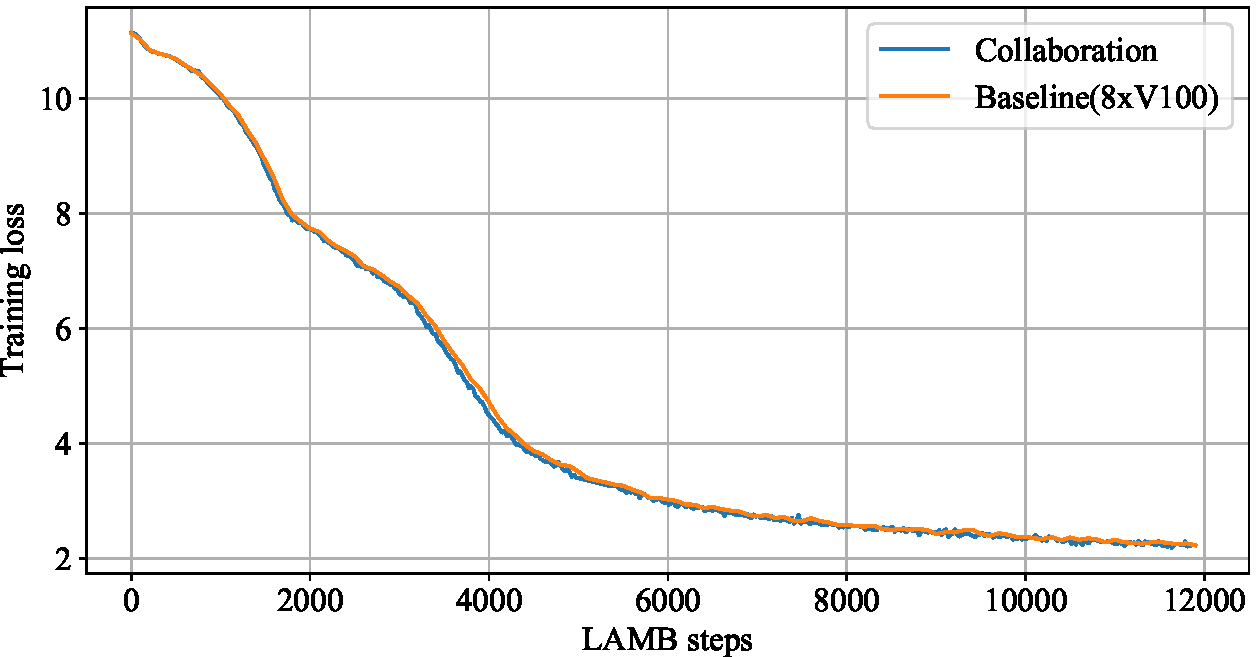
\includegraphics[height=110px]{resources/stepwise_bengali.pdf}
    \caption{Stepwise training progress of DeDLOC and regular distributed training.}
    \label{fig:stepwise_learning_curves}
    \vspace{-12pt}
\end{figure}



\subsection{Training sahajBERT-XL with hybrid GPU + TPU resources}
\label{appendix:xl}

To better explore the practical ramifications of collaborative training, we asked volunteers to train a larger model on the same task as the original sahajBERT. We refer to this model as sahajBERT-XL, as it has approximately the same size as ALBERT-xlarge~\cite{albert}: more specifically, the new model has $d_{model}=2048$, $n_{layers}=24$ and three additional architecture modifications:

\vspace{-4pt}
\begin{itemize}[leftmargin=*]
    \item \textbf{Pre-normalization:} the layer normalization~\cite{ba2016layer} was moved to the beginning of each Transformer layer, as in pre-activation residual networks~\cite{he2016identity}. According to prior work, this modification stabilizes the training process in several Transformer applications~\cite{radford2019language,2020t5}.
    \item \textbf{GeGLU activations:} the new model replaces GeLU activation functions with their gated counterparts known as GeGLU, which were shown to improve the performance of Transformer models~\cite{shazeer2020glu,Narang2021DoTM}. However, unlike~\cite{shazeer2020glu}, sahajBERT-XL uses the same number of GeGLU units as in ALBERT-xlarge, which results in 17M additional parameters.
    \item \textbf{Rotary embeddings:} instead of learned absolute positional embeddings, we equip sahajBERT-XL with rotary embeddings~\cite{su2021roformer} that were recently demonstrated to improve training stability of large language models~\cite{rope-eleutherai}.
\end{itemize}
\vspace{-4pt}

The final model had 72.5M parameters, which is $\approx$4 times more than for original sahajBERT. To reduce the computational requirements of sahajBERT-XL pretraining, we initialized it with Net2Net conversion~\cite{net2net} from the original sahajBERT checkpoint after 10,000 training steps. Because of architectural differences, we needed to manually remove the learned positional embeddings and create a new set of GeGLU parameters, which were initialized by copying the existing pre-GeLU parameters and adding Gaussian noise with the variance of $10^{-3}$. 
We increased the training batch size to 16,384 and used the corresponding learning rate schedule from~\cite{lamb}. Before training, we reaccumulated the LAMB optimizer statistics by running 500 steps with a zero learning rate and setting the training schedule to step 3{,}125, which corresponds to the end of the warmup stage.

Despite using this shortcut, training sahajBERT-XL would still require over 3 months using 8 V100 GPUs. To alleviate this problem, we requested volunteers to use both GPU and preemptible TPU (v2 and v3) instances available in several free-tier cloud providers. As a result, a community of 14 volunteers was able to train sahajBERT-XL in 22 days.

However, training in a hybrid GPU-TPU ``cluster'' has proven challenging due to different mixed precision capabilities. Specifically, the available GPU instances could train in float32 and float16 formats, while the TPU cores support float32 and \textbf{b}float16. Unfortunately, training in float16 on GPU and bfloat16 on TPU caused the model to consistently diverge both with Net2Net initialization and when training from scratch: to combat this issue, we switched TPU computations to float32 while keeping GPU ones in float16. Despite this, a TPUv3-8 peer still outperformed any single GPU node.

Using the techniques described above, the volunteers were able to train a model that outperforms both the baselines and the original sahajBERT model on both downstream tasks (see Table~\ref{tab:downstream}). However, due to the significant computational requirements of sahajBERT-XL, we were only able to train the model once without proper hyperparameter sweeps and ablation analysis. Thus, we believe that future research will reveal more efficient strategies for training with hybrid hardware accelerators.


\subsection{Evaluation}\label{appendix:exp_bengali_evaluation}

We compare sahajBERT with three other pretrained language models: XLM-R~\cite{xlmr}, IndicBert~\cite{kakwani-etal-2020-indicnlpsuite}, and bnRoBERTa~\cite{jain2020indictransformers}. For downstream evaluation, we use two tasks from the Indic General
Language Understanding Evaluation (IndicGLUE) benchmark~\cite{kakwani-etal-2020-indicnlpsuite}: named entity recognition (NER) with the balanced train-dev-test splits version~\cite{rahimi-etal-2019-massively} of the original WikiANN dataset~\cite{pan-etal-2017-cross} and news category classification (NCC) with the Soham News Article dataset~\cite{kakwani-etal-2020-indicnlpsuite}.

Each model was finetuned and evaluated as follows:
\begin{enumerate}[leftmargin=*]
    \item For each combination of learning rate in (1e-5, 3e-5) and the maximum input length in (64, 128, 192, 256, 512), we finetuned the model on each task and computed the validation set metrics to find the best hyperparameters. We computed the F1 score for NER and accuracy for NCC;
    \item For the best configuration, we computed the metrics of the corresponding model on the test set. We repeat this step three times for different random seeds, reporting the mean and the standard deviation of metrics.
\end{enumerate}
All finetuning experiments were run using the Adam~\cite{adam} optimizer with the weight decay fix~\cite{loshchilov2017decoupled}, weight decay of 0.001, and the linear decay learning rate schedule. Finally, each model was trained for a maximum number of 20 epochs and stopped earlier if the loss on the validation set did not decrease during 3 epochs. The size of the batch was chosen to be as large as possible: we started with a batch size of 128 and then, if necessary, the batch size is decreased until it can be stored in memory. For the exact hyperparameter values, see Table~\ref{tab:finetuned-model-hyperparams}.

\begin{table}[t]
\vspace{-16pt}
\caption{Hyperparameter values used for model evaluation.}
\label{tab:finetuned-model-hyperparams}
\centering
\vspace{6pt}
\begin{tabular}{llcccc}
\toprule
       Task     & Model  & Learning rate &  Input length & Batch size  \\
 \multirow{5}{*}{NER} 
 & XLM-R & $10^{-5}$ & 256 & 8 \\
 & IndicBERT & $3\cdot 10^{-5}$ & 256 & 64 \\
 & bnRoBERTa & $3\cdot 10^{-5}$ & 512 & 64 \\
 & sahajBERT & $10^{-5}$ & 128 & 32 \\
 & sahajBERT-XL & $3\cdot 10^{-5}$ & 256 & 64 \\
 \multirow{5}{*}{NCC}
 & XLM-R& $10^{-5}$ & 128 & 8 \\
 & IndicBERT & $3\cdot 10^{-5}$ & 128 & 128 \\
 & bnRoBERTa & $3\cdot 10^{-5}$ & 128 & 64 \\
 & sahajBERT & $3\cdot 10^{-5}$ & 64 & 64 \\
 & sahajBERT-XL & $10^{-5}$ & 128 & 64 \\
\bottomrule
\end{tabular}
\end{table}

\section{Environmental impact} 
\label{appendix:env_impact}
Recent works have outlined the environmental consequences of training ever larger deep learning models~\cite{Strubell2019EnergyAP,Schwartz2020GreenA} and encouraged authors to report the incurred energy costs~\cite{Henderson2020TowardsTS}. The direction proposed in this work may help in two specific ways. First, while most of the current tools focus on the CO$_2$ cost caused by the training-time energy consumption~\cite{Anthony2020CarbontrackerTA}, a more holistic evaluation protocol would need to include the not insignificant manufacturing cost of the training infrastructure~\cite{Kline2016HolisticallyET,Bashroush2018ACR}. The collaborative training method described in this work allows volunteers to make better use of existing computing resources, which helps minimize these costs. Second, the distributed training setting allows users to dispense with the extensive cooling infrastructures required for large concentrated data centers, and may thus also help reduce the operating costs themselves~\cite{Qiu2020CanFL}. We note, however, that the additional networking needs may limit the magnitude of these gains.

\end{document}


